\newpage
{\bfseries IRSTI 87.15.02}

{\bfseries STUDY OF WASTEWATER TREATMENT EFFICIENCY USING A COMBINED METHOD
OF FORWARD AND REVERSE OSMOSIS INTEGRATED WITH ACTIVATED CARBON
TREATMENT}

{\bfseries \textsuperscript{1}K.A. Kurtibay\textsuperscript{🖂},
\textsuperscript{2}Ye.Ye. Zhatkanbayev, \textsuperscript{1}A.
Kappassuly, \textsuperscript{1}A.A. Ussenova,}

{\bfseries \textsuperscript{3}Zh.K. Zhatkanbayeva, \textsuperscript{1}N.B.
Moldagulova, \textsuperscript{1}E.B. Moldagulova}

\textsuperscript{1}«Scientific and Production Center of Ecological and
Industrial Biotechnology» LLP,\\
Astana, Kazakhstan,

\textsuperscript{2}Kazakh University of Technology and Business named
after K. Kulazhanov,\\
Astana, Kazakhstan,

\textsuperscript{3}L.N. Gumilyev Eurasian National University, Astana,
Kazakhstan

{\bfseries \textsuperscript{🖂}}Correspondent-author: kurtibayqb@gmail.com

In Kazakhstan, the issue of providing the population with quality
drinking water remains one of the topical and important issues. Despite
significant efforts in the field of infrastructure and water treatment
technologies, many regions of Kazakhstan still face problems of
pollution and insufficient water resources. In this regard, the
development of effective water treatment methods is of particular
importance. This study considers the issue of wastewater treatment by
the combined method of forward and reverse osmosis, which is a key
direction in modern water treatment. The relevance of the work is the
use of integration of forward osmosis methods with the process of
adsorption by powdered activated carbon in wastewater treatment. The use
of powdered activated carbon in the process of wastewater treatment
leads to a reduction in the content of organic matter, which are water
pollutants. As a result of the experiment with pretreatment of
wastewater with powdered activated carbon, a decrease in the level of
chemical oxygen demand (COD) in wastewater from 538 mg O/dm3 to 256 mg
O/dm3 was observed, as well as a relative decrease in the concentration
of other indicators. The draw solution in the form of 1.5 M NaCl
gradually drawing water molecules from the feed solution pretreated with
activated carbon on the tenth day had a concentration of 0.425 M
absorbing 2.529 liters of water entering through the membrane that is
27.6\% more than the control version of the experiment. The
effectiveness of integrated methods lies in the successful combination
of different technologies to improve water treatment processes and
ensure the availability of clean water not only in Kazakhstan, but also
in different parts of the world.

{\bfseries Key words:} wastewater treatment, forward osmosis, wastewater,
powdered activated carbon, chemical oxygen demand (COD), organic
pollutants, reverse osmosis.

{\bfseries БЕЛСЕНДІРІЛГЕН КӨМІРМЕН ӨҢДЕУМЕН ИНТЕГРАЦИЯЛАНҒАН ТІКЕЛЕЙ ЖӘНЕ
КЕРІ ОСМОС ӘДІСІН ҚОЛДАНА ОТЫРЫП, АҒЫНДЫ СУЛАРДЫ ТАЗАРТУ ТИІМДІЛІГІН
ЗЕРТТЕУ}

{\bfseries \textsuperscript{1}Қ.А. Куртибай\textsuperscript{🖂},
\textsuperscript{2}Е.Е. Жатканбаев, \textsuperscript{1}Ә. Қаппасұлы,
\textsuperscript{1}А.Ә.Үсенова,}

{\bfseries \textsuperscript{3}Ж.К. Жатканбаева, \textsuperscript{1}Н.Б.
Молдагулова, \textsuperscript{1}Э.Б. Молдагулова}

\textsuperscript{1}«Экологиялық және өнеркәсіптік биотехнологияның
ғылыми-өндірістік орталығы» ЖШС,

Астана, Қазақстан,

\textsuperscript{2}Қ. Құлажанов атындағы Қазақ технология және бизнес
университеті,

Астана, Қазақстан,

\textsuperscript{3}Л.Н. Гумилев атындағы Еуразия Ұлттық Университеті,
Астана, Қазақстан,

e-mail: kurtibayqb@gmail.com

Қазақстанда халықты сапалы ауыз сумен қамтамасыз ету мәселесі өзекті
және маңызды мәселелердің бірі болып қала береді. Инфрақұрылым және су
дайындау технологиялары саласындағы елеулі күш-жігерге қарамастан,
Қазақстанның көптеген өңірлері әлі де судың ластануы мен жеткіліксіздігі
проблемаларына тап болып отыр. Осыған байланысты суды тазартудың тиімді
әдістерін жасау ерекше маңызға ие. Бұл зерттеу ағынды суларды тікелей
және кері осмостың аралас әдісімен тазарту мәселесін қарастырады, бұл
қазіргі заманғы суды дайындаудың негізгі бағыты болып табылады. Жұмыстың
өзектілігі ағынды суларды тазарту кезінде ұнтақталған белсендірілген
көмірмен адсорбциялау процесімен тікелей осмос әдістерін интеграциялау
арқылы қолдану болып табылады. Ағынды суларды тазарту процесінде
ұнтақталған белсендірілген көмірді пайдалану суды ластайтын органикалық
заттардың азаюына әкеледі. Ағынды суларды ұнтақталған белсендірілген
көмірмен алдын ала өңдеу экспериментінің нәтижесінде ағынды сулардағы
оттегінің химиялық тұтынылу (ОХТ) деңгейінің 538
мгО/дм\textsuperscript{3}-тен 256 мгО/дм\textsuperscript{3}-ке дейін
төмендеуі, сондай-ақ басқа көрсеткіштер концентрациясының салыстырмалы
төмендеуі байқалады. 1,5 М NaCl түріндегі тартқыш ерітіндісі су
молекулаларын алдын ала белсендірілген көмірмен өңделген бастапқы
ерітіндіден оныншы күні біртіндеп тартып, 0,425 М концентрациясына ие
болып, мембрана арқылы өткен су 2,529 литрді құрады. Бұл эксперименттің
бақылау нұсқасына қарағанда 27,6\% - ға көп. Интеграцияланған әдістердің
тиімділігі суды тазарту процестерін жақсарту және таза судың тек
Қазақстанда ғана емес, әлемнің әр түкпірінде де қолжетімділігін
қамтамасыз ету мақсатында түрлі технологияларды сәтті комбинациялаудан
құралады.

{\bfseries Түйін сөздер:} ағынды суларды тазарту, тікелей осмос, ағынды
сулар, ұнтақталған белсендірілген көмір, оттегінің химиялық тұтынылуы
(ОХТ), органикалық ластаушы заттар, кері осмос.

{\bfseries ИССЛЕДОВАНИЕ ЭФФЕКТИВНОСТИ ОЧИСТКИ СТОЧНЫХ ВОД С ИСПОЛЬЗОВАНИЕМ
КОМБИНИРОВАННОГО МЕТОДА ПРЯМОГО И ОБРАТНОГО ОСМОСА, ИНТЕГРИРОВАННОГО С
ОБРАБОТКОЙ АКТИВИРОВАННЫМ УГЛЕМ}

{\bfseries \textsuperscript{1}Қ.А. Куртибай\textsuperscript{🖂},
\textsuperscript{2}Е.Е. Жатканбаев, \textsuperscript{1}Ә. Қаппасұлы,
\textsuperscript{1}А.Ә. Үсенова,}

{\bfseries \textsuperscript{3}Ж.К. Жатканбаева, \textsuperscript{1}Н.Б.
Молдагулова, \textsuperscript{1}Э.Б. Молдагулова}

\textsuperscript{1} ТОО «Научно-производственный центр экологической и
промышленной биотехнологии»,

Астана, Казахстан,

\textsuperscript{2} Казахский университет технологии и бизнеса имени К.
Кулажанова, Астана, Казахстан,

\textsuperscript{3} Евразийский Национальный Университет имени Л.Н.
Гумилёва, Астана, Казахстан,

e-mail: kurtibayqb@gmail.com

В Казахстане вопрос обеспечения населения качественной питьевой водой
остается одним из актуальных и важных. Несмотря на значительные усилия в
области инфраструктуры и технологий водоподготовки, многие регионы
Казахстана по-прежнему сталкиваются с проблемами загрязнения и
недостаточности водных ресурсов. В связи с этим особое значение
приобретает разработка эффективных методов очистки воды. В данном
исследовании рассматривается вопрос очистки сточных вод комбинированным
методом прямого и обратного осмоса, который является ключевым
направлением в современной водоподготовке. Актуальностью работы является
использование интеграции методов прямого осмоса с процессом адсорбции
порошкообразным активированным углем при очистке сточных вод.
Использование порошкообразного активированного угля в процессе очистки
сточных вод приводит к уменьшению содержания органических веществ,
которые являются загрязняющими воду. В результате эксперимента с
предварительной обработкой сточных вод порошкообразным активированным
углем наблюдается снижение уровня химического потребления кислорода
(ХПК) в сточной воде с 538 мг О/дм3 до 256 мг О/дм3, а также
относительное уменьшение концентрации других показателей. Вытяжной
раствор в виде 1,5 М NaCl постепенно вытягивая молекул воды с исходного
раствора предварительно обработанного активированным углем на десятый
день имел концентрацию 0,425 М поглощая 2,529 литров поступающей через
мембрану воды что на 27,6\% больше, чем на контрольном варианте
эксперимента. Эффективность интегрированных методов заключается в
успешном сочетании различных технологий с целью улучшения процессов
очистки воды и обеспечения доступности чистой воды не только в
Казахстане, но и в различных уголках мира.

{\bfseries Ключевые слова:} очистка сточных вод, прямой осмос, сточные
воды, порошкообразный активированный уголь, химическое потребление
кислорода (ХПК), органические загрязнители, обратный осмос.

{\bfseries Introduction.} In the modern world, the problem of access to
clean drinking water remains one of the most urgent, affecting the
health and well-being of mankind. In Kazakhstan, the issue of providing
the population with quality drinking water remains one of the urgent and
important.

The main pollutants in both natural and polluted water are
microorganisms, as well as organic and inorganic substances. Wastewaters
are solid and liquid substances in water that enter the sewer system as
a by-product of society\textquotesingle s activities. They include
dissolved and suspended organic solids that undergo decomposition or
biodegradation {[}1{]}. Over time, domestic and industrial wastewater
increasingly contains non-biodegradable organic compounds such as humic
substances, which reduce the effectiveness of low-cost wastewater
treatment methods {[}2{]}.

Forward osmosis is used to treat municipal wastewater that is treated in
municipal wastewater treatment plants {[}3{]}. Forward osmosis membrane
systems can remove large ions and concentrate wastewater 10-15 times
{[}4{]}. Forward osmosis can be integrated with reverse osmosis in a
hybrid system. In this case, forward osmosis is used to pre-treat
wastewater to produce high quality water, which is then used to dilute
seawater before the reverse osmosis step. Another study {[}5{]} used a
hybrid process combining direct osmosis and membrane distillation to
remove tetracycline from wastewater. This method provided a purification
rate of 99.9\%, and the water recovery efficiency was 15-22\%. In
addition to water recovery, forward osmosis can be used to treat
wastewater to extract nutrients and generate energy {[}6{]}. Examples of
such recovery include biogas production and recovery of valuable
components such as phosphates, ammonia, and potassium. Moreover, forward
osmosis can help to improve the environmental sustainability of
treatment processes by reducing energy costs and decreasing the burden
on the environment {[}6{]}.

As a result, numerous physicochemical treatment methods such as
coagulation, flocculation, adsorption and accelerated oxidation have
been proposed and investigated for effective wastewater treatment
{[}7{]}. However, physicochemical treatment methods alone are not
sufficient to completely remove various organic pollutants from
wastewater. To address these limitations, the use of membrane filtration
processes in combination with these methods has been proposed. Membrane
filtration methods such as nanofiltration (NF) and reverse osmosis (RO)
have been successfully used for wastewater treatment. However, operation
at high transmembrane pressure increases operating costs and leads to
significant organic fouling of the membrane {[}8,9{]}.

From an economic point of view, the forward osmosis (FO) process is
superior to nanofiltration (NF) and reverse osmosis (RO) due to several
advantages. These advantages include efficient removal of organic and
inorganic contaminants, no need for external hydraulic pressure, and
less membrane fouling with better reversibility {[}10{]}. As previously
stated, the application of membrane filtration techniques in integration
with pretreatment by physicochemical methods such as, coagulation,
flocculation, magnetic ion exchange resins and powdered activated carbon
to avoid membrane fouling shows high efficiency {[}11{]}.

Pretreatment of wastewater to remove organic pollutants with powdered
activated carbon has attracted attention due to its advantages in
conjunction with membrane filtration processes. Powdered activated
carbon provides improved membrane surface cleaning, effective reduction
of irreversible fouling and removal of organic matter.

Currently, biochar stands out as a promising alternative with additional
advantages such as environmental sustainability, low production cost,
soil fertility enhancement and carbon sequestration. Biochar also
possesses additional cationic functional groups, which makes it easy to
modify its surface properties to improve functionality {[}12{]}.

The use of adsorption pretreatment for partial removal of organic
pollutants provides reduction of chemical oxygen demand (COD) of
wastewater.

{\bfseries Methods and Materials.} As an object of study for wastewater
treatment by direct osmosis method, incoming wastewater was taken. The
wastewater sample was collected in the volume of 10 liters at the sewage
treatment plant (STP) located in the vicinity of Astana, Kazakhstan.

To determine the efficiency integrated using powdered activated carbon,
experiments were performed without adsorption step and with pretreatment
with powdered activated carbon for adsorption to investigate a larger
flow of clean water. 1.5 M NaCl was used as a draw solution with higher
osmotic pressure than the stock solution. The concentration of the stock
and draw solutions was measured every 24 hours for 10 days.

\emph{Adsorption of wastewater using powdered activated carbon}

For adsorption, untreated wastewater is filtered through filter paper to
remove coarse suspended solids and the filtrate in a total volume of 500
cm\textsuperscript{3} is placed in Erlenmeyer flasks, then 3.5 g/L
powdered activated carbon is added to the filtrate. The flasks were then
placed on a horizontal shaker for intensive-continuous stirring at 150
r/min for 24 hours at room temperature (25-28°C). During the experiment,
the pH of the solution was maintained at 7 by adding 5M HCl or 5M NaOH
every 4 hours. After adsorption, the solution was filtered through a
paper filter with a pore diameter of 0.45 μm and the resulting filtrate
was stored for the following analyses {[}13{]}. After treatment of the
initial sample by adsorption with powdered activated carbon, a general
physicochemical analysis was performed.

\emph{Physico-chemical methods of research}

\emph{Refractometry.} To determine the concentration of sodium chloride
and sucrose solutions, the refractometry method was used using a
refractometer of Abbemat 350/550 Performance Plus series (Anton Paar,
Austria). All analyses were performed in triplicate.

\emph{Determination of chemical oxygen demand (COD).} COD was measured
according to GOST 31859-2012 ``Water. Method for determination of
chemical oxygen demand'' on the Expert 003 device (spectrophotometer
with thermoreactor). Calibration of the device was carried out with
solutions of the standard sample of chemical oxygen consumption GSO
7552-99. The device has a function of built-in construction of
calibration curve and automatic determination of COD value.

\emph{Determination of chloride ions.} Determination of chloride content
was carried out according to GOST 26425-85 ``Method for determination of
chloride in water extract'', the method of determination - titration by
silver nitrate solution with potassium bichromate indicator.

\emph{Determination of ammonium nitrogen.} Determination of ammonium and
nitrate nitrogen according to GOST 15476-2013 ``Fertilizers.
Determination of nitrate and ammonium nitrogen by the Devard method''.

\emph{Determination of nitrates and nitrites.} Determination of nitrates
and nitrites in water was carried out according to GOST 33045-2014
``Water. Methods of determination of nitrogen-containing substances",
the method of determination by photocalorimetry.

\emph{Determination of phosphate ions.} Determination of phosphate
content in water according to GOST 18309-2014 ``Water. Methods of
determination of phosphorus-containing substances''.

\emph{Determination of suspended solids.} Suspended solids were
determined according to PND F 14.1:2:4.254-09 ``Methods of measuring
mass concentrations of suspended and calcined suspended solids in
drinking, natural and waste water samples by gravimetric method''.

\emph{Processing of the obtained results}

The osmotic pressure of solutions with known concentration was
determined by the osmotic pressure (π) Vant-Goff equation:

\begin{longtable}[]{@{}
  >{\raggedright\arraybackslash}p{(\columnwidth - 2\tabcolsep) * \real{0.9470}}
  >{\raggedright\arraybackslash}p{(\columnwidth - 2\tabcolsep) * \real{0.0530}}@{}}
\toprule\noalign{}
\begin{minipage}[b]{\linewidth}\raggedright
\[\pi = C(x)RT\]
\end{minipage} & \begin{minipage}[b]{\linewidth}\raggedright
(1)
\end{minipage} \\
\midrule\noalign{}
\endhead
\bottomrule\noalign{}
\endlastfoot
\end{longtable}

The osmotic pressure gradient of the initial and extraction solutions
was determined by the equation:

\begin{longtable}[]{@{}
  >{\raggedright\arraybackslash}p{(\columnwidth - 2\tabcolsep) * \real{0.9470}}
  >{\raggedright\arraybackslash}p{(\columnwidth - 2\tabcolsep) * \real{0.0530}}@{}}
\toprule\noalign{}
\begin{minipage}[b]{\linewidth}\raggedright
\[\mathrm{\Delta}\pi = \ \pi_{DS} - \pi_{FS}\]
\end{minipage} & \begin{minipage}[b]{\linewidth}\raggedright
(2)
\end{minipage} \\
\midrule\noalign{}
\endhead
\bottomrule\noalign{}
\endlastfoot
\end{longtable}

Water flux is determined by water transport across the semipermeable
membrane due to osmotic pressure difference by equation {[}14{]}:

\begin{longtable}[]{@{}
  >{\raggedright\arraybackslash}p{(\columnwidth - 2\tabcolsep) * \real{0.9470}}
  >{\raggedright\arraybackslash}p{(\columnwidth - 2\tabcolsep) * \real{0.0530}}@{}}
\toprule\noalign{}
\begin{minipage}[b]{\linewidth}\raggedright
\[J_{w} = A(\pi_{DS} - \pi_{FS})\]
\end{minipage} & \begin{minipage}[b]{\linewidth}\raggedright
(3)
\end{minipage} \\
\midrule\noalign{}
\endhead
\bottomrule\noalign{}
\endlastfoot
\end{longtable}

The analysis and processing of the obtained data was carried out through
calculations and equations, and visualizations in the form of graphs and
charts were constructed using Microsoft Excel software (Office 16)

{\bfseries Results and discussion.} Before the beginning of all experiments
the initial general physico-chemical analysis of the selected sample of
incoming wastewater of the sewage treatment plant of Astana city was
carried out. All chemical analyses were carried out in accordance with
the State standards. The results of the general physico-chemical
analysis are given in Table 1.

{\bfseries Table 1 - Indicators of physico-chemical analysis of incoming
wastewater of the sewage treatment plant of Astana city}

\begin{longtable}[]{@{}
  >{\raggedright\arraybackslash}p{(\columnwidth - 2\tabcolsep) * \real{0.5305}}
  >{\raggedright\arraybackslash}p{(\columnwidth - 2\tabcolsep) * \real{0.4695}}@{}}
\toprule\noalign{}
\begin{minipage}[b]{\linewidth}\raggedright
Name of physico-chemical parameters
\end{minipage} & \begin{minipage}[b]{\linewidth}\raggedright
Results
\end{minipage} \\
\midrule\noalign{}
\endhead
\bottomrule\noalign{}
\endlastfoot
pH & 7,83 \\
Temperature & 22 \\
COD, mg O/dm\textsuperscript{3} & 538 \\
Suspended solids, mg/ dm\textsuperscript{3} & 2584 \\
Phosphorus (РO\textsubscript{4}), mg/ dm\textsuperscript{3} & 3,69 \\
Ammonium nitrogen, mg/ dm\textsuperscript{3} & 18,34 \\
Nitrite nitrogen, mg/ dm\textsuperscript{3} & 1,51 \\
Nitrate nitrogen, mg/ dm\textsuperscript{3} & 8,26 \\
Chlorides, mg/ dm\textsuperscript{3} & 13,2 \\
Ash content, \% & 128 \\
\end{longtable}

According to the results of the general physico-chemical analysis we can
notice a high level of water pollution by organic substances, which is
estimated by the value of chemical oxygen demand (COD) of the object
under study. In this case, the incoming wastewater of the sewage
treatment plant of Astana city has COD - 538 mg O/dm3. Also relatively
high content of nitrate, nitrite, ammonium, phosphate and chloride ions,
exceeding the maximum permissible concentration (MPC). The hydrogen
index of this wastewater is 7.83, which characterizes the alkalinity of
this sample.

\emph{Adsorption of wastewater using powdered activated carbon}

For adsorption, the untreated wastewater is filtered through filter
paper to remove coarse suspended solids and the filtrate in a total
volume of 500 cm3 is placed in Erlenmeyer flasks, then 3.5 g/L powdered
activated carbon is added to the filtrate. The flasks were then placed
on a horizontal shaker for intensive-continuous stirring at 150 r/min
for 24 hours at room temperature (25-28°C). During the experiment, the
pH of the solution was maintained at 7 by adding 5M HCl or 5M NaOH every
4 hours. After adsorption, the solution was filtered through a paper
filter with a pore diameter of 0.45 μm and the resulting filtrate was
stored for the following analyses {[}13{]}. After treatment of the
initial sample by adsorption with powdered activated carbon, a general
physicochemical analysis was carried out.

The results obtained after adsorption are shown in Table 2.

{\bfseries Table 2 - Indicators of general physicochemical analysis after
adsorption}

\begin{longtable}[]{@{}
  >{\raggedright\arraybackslash}p{(\columnwidth - 2\tabcolsep) * \real{0.6654}}
  >{\raggedright\arraybackslash}p{(\columnwidth - 2\tabcolsep) * \real{0.3346}}@{}}
\toprule\noalign{}
\begin{minipage}[b]{\linewidth}\raggedright
Name of physico-chemical parameters
\end{minipage} & \begin{minipage}[b]{\linewidth}\raggedright
Results
\end{minipage} \\
\midrule\noalign{}
\endhead
\bottomrule\noalign{}
\endlastfoot
pH & 7,71 \\
Temperature & 25 \\
COD, mg O/dm\textsuperscript{3} & 256 \\
Suspended solids, mg/ dm\textsuperscript{3} & 367 \\
Phosphorus (РO\textsubscript{4}), mg/ dm\textsuperscript{3} & 3,25 \\
Ammonium nitrogen, mg/ dm\textsuperscript{3} & 17,67 \\
Nitrite nitrogen, mg/ dm\textsuperscript{3} & 1,42 \\
Nitrate nitrogen, mg/ dm\textsuperscript{3} & 8,11 \\
Chlorides, mg/ dm\textsuperscript{3} & 12,84 \\
Ash content, \% & 84 \\
\end{longtable}

According to the results obtained after the analysis with pretreatment
with powdered activated carbon we can observe a decrease in COD level of
wastewater from 538 mg O/dm3 to 256 mg O/dm3. And also, relative
decrease of concentration of other indicators.

\emph{Integration of the adsorption process with a forward osmosis
system}

The forward osmosis system used was a plant that was designed for
desalination of sea salt water. The process of concentrating wastewater
to produce clean secondary water was carried out in a similar way to the
forward osmosis desalination method, since the basic principle of this
method is the same for all types of treatment, recovery and
concentration. The methods differ only in that, depending on the
purpose, chemical composition, concentration and osmotic pressure of the
feed solution, different draw solutions are used, respectively higher
osmotic pressure than the feed solution for greater water flux through
the semipermeable membrane. And also, different membranes of different
nature are applied relative to the purpose of the solution.

To determine the efficiency integrated using powdered activated carbon,
experiments were performed without adsorption step and with pretreatment
with powdered activated carbon for adsorption to investigate the higher
flow of pure water. 1.5 M NaCl was used as a draw solution with higher
osmotic pressure than the feed solution. Concentration measurements of
feed and draw solutions were made every 24 hours for 10 days. The water
flux was measured by evaluating the change in concentration and osmotic
pressure of sodium chloride in the feed and draw solutions, as well as
the change in the volume of solution in the draw solution compartment.
The concentration of sodium chloride was measured by refractometry.

The results of experiments on water treatment by forward osmosis method
without pretreatment and by complex method are given in Tables 3-4.

{\bfseries Table 3 - Wastewater treatment by forward osmosis without
pretreatment with powdered}

{\bfseries activated carbon}

\begin{longtable}[]{@{}
  >{\raggedright\arraybackslash}p{(\columnwidth - 18\tabcolsep) * \real{0.2519}}
  >{\raggedright\arraybackslash}p{(\columnwidth - 18\tabcolsep) * \real{0.0768}}
  >{\raggedright\arraybackslash}p{(\columnwidth - 18\tabcolsep) * \real{0.1172}}
  >{\raggedright\arraybackslash}p{(\columnwidth - 18\tabcolsep) * \real{0.0017}}
  >{\raggedright\arraybackslash}p{(\columnwidth - 18\tabcolsep) * \real{0.1177}}
  >{\raggedright\arraybackslash}p{(\columnwidth - 18\tabcolsep) * \real{0.0012}}
  >{\raggedright\arraybackslash}p{(\columnwidth - 18\tabcolsep) * \real{0.1189}}
  >{\raggedright\arraybackslash}p{(\columnwidth - 18\tabcolsep) * \real{0.1189}}
  >{\raggedright\arraybackslash}p{(\columnwidth - 18\tabcolsep) * \real{0.1189}}
  >{\raggedright\arraybackslash}p{(\columnwidth - 18\tabcolsep) * \real{0.0767}}@{}}
\toprule\noalign{}
\begin{minipage}[b]{\linewidth}\raggedright
Time, days
\end{minipage} & \begin{minipage}[b]{\linewidth}\raggedright
0
\end{minipage} & \begin{minipage}[b]{\linewidth}\raggedright
2
\end{minipage} &
\multicolumn{2}{>{\raggedright\arraybackslash}p{(\columnwidth - 18\tabcolsep) * \real{0.1194} + 2\tabcolsep}}{%
\begin{minipage}[b]{\linewidth}\raggedright
4
\end{minipage}} &
\multicolumn{2}{>{\raggedright\arraybackslash}p{(\columnwidth - 18\tabcolsep) * \real{0.1201} + 2\tabcolsep}}{%
\begin{minipage}[b]{\linewidth}\raggedright
6
\end{minipage}} & \begin{minipage}[b]{\linewidth}\raggedright
8
\end{minipage} & \begin{minipage}[b]{\linewidth}\raggedright
10
\end{minipage} & \begin{minipage}[b]{\linewidth}\raggedright
\end{minipage} \\
\midrule\noalign{}
\endhead
\bottomrule\noalign{}
\endlastfoot
COD, mg O/dm\textsuperscript{3} & 538 & 1216 &
\multicolumn{2}{>{\raggedright\arraybackslash}p{(\columnwidth - 18\tabcolsep) * \real{0.1194} + 2\tabcolsep}}{%
1932} &
\multicolumn{2}{>{\raggedright\arraybackslash}p{(\columnwidth - 18\tabcolsep) * \real{0.1201} + 2\tabcolsep}}{%
2367} & 2527 & 2714 & \\
NO\textsubscript{3}\textsuperscript{3-}, mg O/dm\textsuperscript{3} &
8,26 & 18,66 &
\multicolumn{2}{>{\raggedright\arraybackslash}p{(\columnwidth - 18\tabcolsep) * \real{0.1194} + 2\tabcolsep}}{%
29,96} &
\multicolumn{2}{>{\raggedright\arraybackslash}p{(\columnwidth - 18\tabcolsep) * \real{0.1201} + 2\tabcolsep}}{%
36,70} & 39,18 & 42,08 & \\
NH\textsubscript{4}\textsuperscript{4+}, mg O/dm\textsuperscript{3} &
18,34 & 41,45 &
\multicolumn{2}{>{\raggedright\arraybackslash}p{(\columnwidth - 18\tabcolsep) * \real{0.1194} + 2\tabcolsep}}{%
66,52} &
\multicolumn{2}{>{\raggedright\arraybackslash}p{(\columnwidth - 18\tabcolsep) * \real{0.1201} + 2\tabcolsep}}{%
81,48} & 86,99 & 93,43 & \\
PO\textsubscript{4}\textsuperscript{3-}, mg O/dm\textsuperscript{3} &
3,69 & 8,34 &
\multicolumn{2}{>{\raggedright\arraybackslash}p{(\columnwidth - 18\tabcolsep) * \real{0.1194} + 2\tabcolsep}}{%
13,38} &
\multicolumn{2}{>{\raggedright\arraybackslash}p{(\columnwidth - 18\tabcolsep) * \real{0.1201} + 2\tabcolsep}}{%
16,39} & 17,50 & 18,80 & \\
NO\textsubscript{2}\textsuperscript{2-}, mg O/dm\textsuperscript{3} &
1,51 & 3,41 &
\multicolumn{2}{>{\raggedright\arraybackslash}p{(\columnwidth - 18\tabcolsep) * \real{0.1194} + 2\tabcolsep}}{%
5,47} &
\multicolumn{2}{>{\raggedright\arraybackslash}p{(\columnwidth - 18\tabcolsep) * \real{0.1201} + 2\tabcolsep}}{%
6,70} & 7,16 & 7,69 & \\
Cl\textsuperscript{-}, mg O/dm\textsuperscript{3} & 13,2 & 29,81 &
\multicolumn{2}{>{\raggedright\arraybackslash}p{(\columnwidth - 18\tabcolsep) * \real{0.1194} + 2\tabcolsep}}{%
47,82} &
\multicolumn{2}{>{\raggedright\arraybackslash}p{(\columnwidth - 18\tabcolsep) * \real{0.1201} + 2\tabcolsep}}{%
58,57} & 62,59 & 67,22 & \\
Concentration of draw solution, mol/L & 1,500 &
\multicolumn{2}{>{\raggedright\arraybackslash}p{(\columnwidth - 18\tabcolsep) * \real{0.1189} + 2\tabcolsep}}{%
1,252} &
\multicolumn{2}{>{\raggedright\arraybackslash}p{(\columnwidth - 18\tabcolsep) * \real{0.1189} + 2\tabcolsep}}{%
1,128} & 0,985 & 0,912 & 0,884 & \\
Osmotic pressure of draw solution π, Pa & -- &
\multicolumn{2}{>{\raggedright\arraybackslash}p{(\columnwidth - 18\tabcolsep) * \real{0.1189} + 2\tabcolsep}}{%
3,102*10\textsuperscript{3}} &
\multicolumn{2}{>{\raggedright\arraybackslash}p{(\columnwidth - 18\tabcolsep) * \real{0.1189} + 2\tabcolsep}}{%
2,795*10\textsuperscript{3}} & 2,440*10\textsuperscript{3} &
2,260*10\textsuperscript{3} & 2,143*10\textsuperscript{3} & \\
Gradient of osmotic pressure Δπ, Pa & -- &
\multicolumn{2}{>{\raggedright\arraybackslash}p{(\columnwidth - 18\tabcolsep) * \real{0.1189} + 2\tabcolsep}}{%
2,054*10\textsuperscript{3}} &
\multicolumn{2}{>{\raggedright\arraybackslash}p{(\columnwidth - 18\tabcolsep) * \real{0.1189} + 2\tabcolsep}}{%
1,850*10\textsuperscript{3}} & 1,616*10\textsuperscript{3} &
1,497*10\textsuperscript{3} & 1,450*10\textsuperscript{3} & \\
Water flux Jw, L*m\textsuperscript{-2}*h\textsuperscript{-1} & -- &
\multicolumn{2}{>{\raggedright\arraybackslash}p{(\columnwidth - 18\tabcolsep) * \real{0.1189} + 2\tabcolsep}}{%
20,54} &
\multicolumn{2}{>{\raggedright\arraybackslash}p{(\columnwidth - 18\tabcolsep) * \real{0.1189} + 2\tabcolsep}}{%
18,50} & 16,15 & 14,97 & 14,50 & \\
Volume of clean water, ml & -- &
\multicolumn{2}{>{\raggedright\arraybackslash}p{(\columnwidth - 18\tabcolsep) * \real{0.1189} + 2\tabcolsep}}{%
0,198} &
\multicolumn{2}{>{\raggedright\arraybackslash}p{(\columnwidth - 18\tabcolsep) * \real{0.1189} + 2\tabcolsep}}{%
0,131} & 0,198 & 0,122 & 0,054 & \\
\end{longtable}

{\bfseries Table 4 - Wastewater treatment by integrated forward osmosis
method with pretreatment}

{\bfseries with powdered activated carbon}

\begin{longtable}[]{@{}
  >{\raggedright\arraybackslash}p{(\columnwidth - 12\tabcolsep) * \real{0.3261}}
  >{\raggedright\arraybackslash}p{(\columnwidth - 12\tabcolsep) * \real{0.0676}}
  >{\raggedright\arraybackslash}p{(\columnwidth - 12\tabcolsep) * \real{0.1213}}
  >{\raggedright\arraybackslash}p{(\columnwidth - 12\tabcolsep) * \real{0.1213}}
  >{\raggedright\arraybackslash}p{(\columnwidth - 12\tabcolsep) * \real{0.1213}}
  >{\raggedright\arraybackslash}p{(\columnwidth - 12\tabcolsep) * \real{0.1213}}
  >{\raggedright\arraybackslash}p{(\columnwidth - 12\tabcolsep) * \real{0.1213}}@{}}
\toprule\noalign{}
\begin{minipage}[b]{\linewidth}\raggedright
Time, days
\end{minipage} & \begin{minipage}[b]{\linewidth}\raggedright
0
\end{minipage} & \begin{minipage}[b]{\linewidth}\raggedright
2
\end{minipage} & \begin{minipage}[b]{\linewidth}\raggedright
4
\end{minipage} & \begin{minipage}[b]{\linewidth}\raggedright
6
\end{minipage} & \begin{minipage}[b]{\linewidth}\raggedright
8
\end{minipage} & \begin{minipage}[b]{\linewidth}\raggedright
10
\end{minipage} \\
\midrule\noalign{}
\endhead
\bottomrule\noalign{}
\endlastfoot
COD, mg O/dm\textsuperscript{3} & 256 & 1024 & 1792 & 2612 & 2965 &
3288 \\
NO\textsubscript{3}\textsuperscript{3-}, mg O/dm\textsuperscript{3} &
8,11 & 32,44 & 56,77 & 82,75 & 93,9 & 104,16 \\
NH\textsubscript{4}\textsuperscript{4+}, mg O/dm\textsuperscript{3} &
17,67 & 70,68 & 123,69 & 180,29 & 204,58 & 226,94 \\
PO\textsubscript{4}\textsuperscript{3-}, mg O/dm\textsuperscript{3} &
3,25 & 13,0 & 22,75 & 33,16 & 37,63 & 41,74 \\
NO\textsubscript{2}\textsuperscript{2-}, mg O/dm\textsuperscript{3} &
1,42 & 5,68 & 9,94 & 14,48 & 16,43 & 18,23 \\
Cl\textsuperscript{-}, mg O/dm\textsuperscript{3} & 12,84 & 51,36 &
89,88 & 130,93 & 148,56 & 167,84 \\
Concentration of draw solution, mol/L & 1,500 & 1,056 & 0,884 & 0,693 &
0,512 & 0,425 \\
Osmotic pressure of draw solution π, Pa & -- &
2,616*10\textsuperscript{3} & 2,190*10\textsuperscript{3} &
1,717*10\textsuperscript{3} & 1,269*10\textsuperscript{3} &
1,053*10\textsuperscript{3} \\
Gradient of osmotic pressure Δπ, Pa & -- & 2,386*10\textsuperscript{3} &
1,998*10\textsuperscript{3} & 1,566*10\textsuperscript{3} &
1,157*10\textsuperscript{3} & 0,961*10\textsuperscript{3} \\
Water flux Jw, L*m\textsuperscript{-2}*h\textsuperscript{-1} & -- &
23,86 & 19,98 & 15,66 & 11,57 & 9,61 \\
Volume of clean water, ml & -- & 0,420 & 0,249 & 0,498 & 0,763 &
0,599 \\
\end{longtable}

A forward osmosis system without adsorbent pretreatment of the feed
solution was taken into consideration as a control for this experiment,
which allowed us to compare the water flux through the membrane and
membrane fouling potential with the integrated forward osmosis method
with pre-adsorption by powdered activated carbon.

The integrated method with pre-adsorption with powdered activated carbon
resulted in a significant increase in the maximum water flux, which is
observed after 2 days from the beginning of the experiment compared to
the control by 16.17\%. In addition, judging by the results obtained, it
can be seen that after pretreatment of wastewater with activated carbon,
the membrane fouling potential decreases, at the expense of this
wastewater in the compartment for feed water is more quickly
concentrated losing water molecules, and the draw solution is diluted
reducing its osmotic pressure to the onset of osmotic pressure
equilibrium in the two compartments. The draw solution in the form of
1.5 M NaCl gradually drawing water molecules from the feed solution on
day 10 had a concentration of 0.425 M absorbing 2.529 liters of water
entering through the membrane, which is 27.6\% more than the control
version of the experiment.

Concentrated wastewater with a significantly higher content of organic
matter can serve as an alternative substrate for anaerobic digestion
{[}15{]}, most often carried out for biogas production. The high content
of organic matter in concentrated wastewater is evidenced by COD values,
which reached 2714 mg O/dm3 in the control, and in the experiment with
pretreatment due to high water flux concentrated to 3288 mg O/dm3
despite the fact that during adsorption part of the organic matter
remained on the sorbent.

\emph{Pure water recovery by reverse osmosis method}

To obtain clean secondary water for domestic and agricultural use, a
number of methods are used today. One of these methods is the reverse
osmosis method. In comparison with forward osmosis, reverse osmosis has
a number of disadvantages such as high energy consumption, high degree
of membrane fouling, scaling, etc. Therefore, modern researchers have
proposed a hybrid method ``FO-RO'', a method of forward and reverse
osmosis {[}16{]}.

After completion of wastewater treatment by forward osmosis, a dilute
draw solution remains from which pure water must be extracted.
Extraction of pure water by thermal distillation requires a lot of
electrical energy and takes more time. Thus, it was decided to recover
pure water from dilute solutions using «Atoll» reverse osmosis systems
with a pure water flux capacity of 7.5 liters per hour.

{\bfseries Conclusions.} Application of adsorption method by powdered
activated carbon in wastewater treatment allows to reduce the
concentration of organic substances that pollute water. According to the
results of the experiment with pretreatment of wastewater with powdered
activated carbon we can observe a decrease in the level of COD of
wastewater from 538 mgO/dm3 to 256 mgO/dm3. As well as a relative
decrease in the concentration of other indicators.

The use of the integrated method of pre-adsorption of wastewater by
powdered activated carbon led to a significant increase in the maximum
water flux, which is observed after 2 days from the beginning of the
experiment compared to the control by 16.17\%. In addition, judging by
the results obtained, it can be seen that after pretreatment of
wastewater with activated carbon, the membrane fouling potential
decreases, at the expense of this wastewater in the compartment for feed
water is more quickly concentrated losing water molecules, and the draw
solution is diluted reducing its osmotic pressure to the onset of
osmotic pressure equilibrium in the two compartments. The draw solution
in the form of 1.5 M NaCl gradually drawing water molecules from the
feed solution on day 10 had a concentration of 0.425 M absorbing 2.529
liters of water entering through the membrane, which is 27.6\% more than
the control version of the experiment. After completion of wastewater
treatment by forward osmosis method, there remains a dilute draw
solution from which pure water should be extracted. Extraction of pure
water by thermal distillation requires a lot of electricity and takes
more time. Therefore, it was decided to recover pure water from diluted
solutions by reverse osmosis method using reverse osmosis systems
«Atoll», the capacity of pure water flux of 7.5 l/h. Which proves the
effectiveness of the combined method «FO-RO».

Thus, the results obtained at the end of the experiments indicate that
wastewater treatment using the forward osmosis method, as well as the
integration of this process with the activated carbon adsorption method,
represent a cost-effective and efficient approach to obtaining clean
water for reuse in various industries and agriculture. These integrated
methods can successfully combine different technologies to improve water
treatment processes and increase the availability of clean water not
only in Kazakhstan, but also in other regions of the world.

{\bfseries References}

\begin{enumerate}
\def\labelenumi{\arabic{enumi}.}
\item
  Sonune A., Ghate R. Developments in wastewater treatment methods
  //Desalination. -- 2004. -Vol. 167. -P. 55-63. DOI
  10.1016/j.desal.2004.06.113
\item
  Da Costa F. M. et al. Evaluation of the biodegradability and toxicity
  of landfill leachates after pretreatment using advanced oxidative
  processes //Waste management.-2018. -Vol. 76.- P. 606-613. DOI
  10.1016/j.wasman.2018.02.030
\item
  Hey, T., Bajraktari, N., Davidsson, Å., Vogel, J., Madsen, H. T.,
  Hélix-Nielsen, C., ... \& Jönsson, K. Evaluation of direct membrane
  filtration and direct forward osmosis as concepts for compact and
  energy-positive municipal wastewater treatment //Environmental
  technology.- 2018. -Vol. 39(3).- P. 264-276. DOI
  10.1080/09593330.2017.1298677
\item
  Gao, Y., Fang, Z., Liang, P., \& Huang, X. Direct concentration of
  municipal sewage by forward osmosis and membrane fouling behavior
  //Bioresource technology. -2018. -Vol. 247.-P. 730-735. DOI
  10.1016/j.biortech.2017.09.145
\item
  Pan, S. F., Dong, Y., Zheng, Y. M., Zhong, L. B., \& Yuan, Z. H.
  Self-sustained hydrophilic nanofiber thin film composite forward
  osmosis membranes: Preparation, characterization and application for
  simulated antibiotic wastewater treatment //Journal of Membrane
  Science.- 2017. -Vol. 523.- P. 205-215.
\item
  Ansari, A. J., Hai, F. I., Price, W. E., Drewes, J. E., \& Nghiem, L.
  D. Forward osmosis as a platform for resource recovery from municipal
  wastewater-A critical assessment of the literature //Journal of
  membrane science.-2017. -Vol. 529.-P. 195-206. DOI
  10.1016/j.memsci.2017.01.054
\item
  Liu Z. P. et al. Characterization of dissolved organic matter in
  landfill leachate during the combined treatment process of air
  stripping, Fenton, SBR and coagulation //Waste Management. - 2015.
  -Vol. 41. -P. 111-118. DOI 10.1016/j.wasman.2015.03.044
\item
  Oloibiri V. et al. Characterisation of landfill leachate by
  EEM-PARAFAC-SOM during physical-chemical treatment by
  coagulation-flocculation, activated carbon adsorption and ion exchange
  //Chemosphere.-2017. -Vol.186.-P. 873-883. DOI
  10.1016/j.chemosphere.2017.08.035
\end{enumerate}

Šír M. et al. The effect of humic acids on the reverse osmosis treatment
of hazardous landfill leachate //Journal of Hazardous
Materials.-2012.-Vol.207.- P.86-90.

DOI 10.1016/j.jhazmat.2011.08.079

\begin{enumerate}
\def\labelenumi{\arabic{enumi}.}
\setcounter{enumi}{8}
\item
  Iskander S. M. et al. Energy consumption by forward osmosis treatment
  of landfill leachate for water recovery //Waste Management.-2017.
  -Vol.63.- P. 284-291.
\end{enumerate}

DOI 10.1016/j.wasman.2017.03.026

\begin{enumerate}
\def\labelenumi{\arabic{enumi}.}
\setcounter{enumi}{9}
\item
  Dolar D., Košutić K., Strmecky T. Hybrid processes for treatment of
  landfill leachate: coagulation/UF/NF-RO and adsorption/UF/NF-RO
  //Separation and purification technology. -- 2016.-Vol.168.- P. 39-46.
  DOI 10.1016/j.seppur.2016.05.016
\item
  Rajapaksha A. U. et al. Engineered/designer biochar for contaminant
  removal/immobilization from soil and water: potential and implication
  of biochar modification //Chemosphere. -2016. -Vol.148.-P. 276-291.
  DOI 10.1016/j.chemosphere.2016.01.043
\item
  Aftab B. et al. Targeted removal of organic foulants in landfill
  leachate in forward osmosis system integrated with biochar/activated
  carbon treatment //Water research. -2019. -Vol.160.-P. 217-227. DOI
  10.1016/j.watres.2019.05.076
\item
  Darwish M. A. et al. The forward osmosis and desalination
  //Desalination and Water Treatment. - 2016. -Vol. 57(10).-P.
  4269-4295. DOI 10.1080/19443994.2014.995140
\item
  Chen L. et al. Performance of a submerged anaerobic membrane
  bioreactor with forward osmosis membrane for low-strength wastewater
  treatment //Water research.- 2014.-Vol.50. -P. 114 -123. DOI
  10.1016/j.watres.2013.12.009
\item
  Bamaga O. A. et al. Hybrid FO/RO desalination system: Preliminary
  assessment of osmotic energy recovery and designs of new FO membrane
  module configurations //Desalination. - 2011. -Vol. 268(1-3).- P.
  163-169. DOI 10.1016/j.desal.2010.10.013
\end{enumerate}

\emph{{\bfseries Information about the authors}}

Kurtibay K.A. - Master\textquotesingle s student, Research Associate of
«Scientific and Production Center of Ecological and Industrial
Biotechnology» LLP, Astana, Kazakhstan, e-mail: kurtibayqb@gmail.com;

Zhatkanbayev Ye.Ye. - Doctor of Technical Sciences, Associate Professor,
Kazakh University of Technology and Business named after K. Kulazhanov,
Astana, Kazakhstan, e-mail: erlan.ntp@mail.ru;

Kappassuly A. - Master of Engineering and Technology, Research
Associate, «Scientific and Production Center of Ecological and
Industrial Biotechnology» LLP, Astana, Kazakhstan, e-mail:
kappasuly@mail.ru;

Ussenova A.A. - Master of Natural Sciences, General Director,
«Scientific and Production Center of Ecological and Industrial
Biotechnology» LLP, Astana, Kazakhstan, e-mail: ussenovaaall@gmail.com;

Zhatkanbayeva Zh.K. - Candidate of Chemical Sciences, Associate
Professor, L.N. Gumilev Eurasian National University, Astana,
Kazakhstan, e-mail: zhanna01011973@mail.ru;

Moldagulova N.B. - Candidate of Veterinary Sciences, Leading Researcher,
«Scientific and Production Center of Ecological and Industrial
Biotechnology» LLP, Astana, Kazakhstan, e-mail: m\_nazira1967@mail.ru;

Moldagulova E.B. - junior researcher, «Scientific and Production Center
of Ecological and Industrial Biotechnology» LLP, Astana, Kazakhstan,
e-mail: molgagulova\_elmira1968@mail.ru.

\emph{{\bfseries Сведения об авторах}}

Куртибай Қ.А.- магистрант, научный сотрудник ТОО
«Научно-производственный центр экологической и промышленной
биотехнологии», Астана, Казахстан, e-mail: kurtibayqb@gmail.com;

Жатканбаев Е.Е. - д.т.н., ассоциированный профессор, Казахский
университет технологии и бизнеса имени К. Кулажанова, Астана, Казахстан,
e-mail: erlan.ntp@mail.ru;

Қаппасұлы Ә. -магистр техники и технологии, научный сотрудник ТОО
«Научно-производственный центр экологической и промышленной
биотехнологии», Астана, Казахстан, e-mail: kappasuly@mail.ru;

Үсенова А.Ә. - магистр естествознания, генеральный директор ТОО
«Научно-производственный центр экологической и промышленной
биотехнологии», Астана, Казахстан, e-mail: ussenovaaall@gmail.com;

Жатканбаева Ж.К. - к.х.н., доцент, Евразийский Национальный Университет
имени Л.Н. Гумилева, Астана, Казахстан, e-mail: zhanna01011973@mail.ru;

Молдагулова Н.Б. - к.в.н, ведущий научный сотрудник ТОО
«Научно-производственный центр экологической и промышленной
биотехнологии», Астана, Казахстан, e-mail: m\_nazira1967@mail.ru;

Молдагулова Э.Б.-младший научный сотрудник ТОО «Научно-производственный
центр экологической и промышленной биотехнологии», Астана, Казахстан,
e-mail: molgagulova\_elmira1968@mail.ru.

{\bfseries SRSTI 53.37.13}

{\bfseries STUDY OF THE BEHAVIOR OF ARSENIC IN COPPER ELECTROLYTE}

{\bfseries Kh.B. Omarov\textsuperscript{🖂}, Zh.T. Nurtai, N.U.
Nurgaliev\textsuperscript{🖂}, A.Kh Takirova}

K.Kulazhanov named Kazakh University of Technology and Business,

Astana, Kazakhstan,

{\bfseries \textsuperscript{🖂}}Correspondent-author: homarov1963@mail.ru,
nurgaliev\_nao@mail.ru

In industrial wastewater, arsenic is most often present in the trivalent
state. An analysis of existing purification methods shows that in all
cases, with a few exceptions, the most complete removal of arsenic is
observed from solutions in which it is in the pentavalent state. This is
explained by the significantly lower solubility of arsenates of heavy
and alkaline earth metals compared to the corresponding arsenites. The
chemical oxidation of As(III) in the following systems was studied:
As(III)-H\textsubscript{2}SO\textsubscript{4}-H\textsubscript{2}O,
As(III)-MeSO\textsubscript{4}-H\textsubscript{2}O,
As(III)--H\textsubscript{2}SO\textsubscript{4}--MeSO\textsubscript{4}--H\textsubscript{2}O
(where Me is Cu, Ni, Co, Mn, Zn). The influence of temperature, the
amount of transition metal ions, the duration of the experiment, and the
concentration of sulfuric acid on the degree of transition of As(III) to
As(V) was studied. The effect of catalytic oxidation of As(III) in
sulfuric acid solutions was discovered. The maximum degree of oxidation
of trivalent arsenic (55-60\%) is observed when transition metal salts
are introduced into an arsenic solution in the presence of a platinum
plate. It has been established that the nature of the studied transition
metal salts (Cu\textsuperscript{2+}, Ni\textsuperscript{2+},
Co\textsuperscript{2+}, Mn\textsuperscript{2+}, Zn\textsuperscript{2+}),
process duration and temperature do not have a significant effect on the
degree of As(III) conversion. The results obtained largely explain the
predominance of pentavalent forms of arsenic in production solutions of
non-ferrous metallurgy.

{\bfseries Keywords:} copper electrolyte, arsenic, transition metals,
catalytic role, instant oxidation effect, activated oxygen.

{\bfseries МЫС ЭЛЕКТРОЛИТІНДЕГІ МЫШЬЯКТІҢ КҮЙІН ЗЕРТТЕУ}

{\bfseries Х.Б. Омаров\textsuperscript{🖂}, Ж.Т. Нұртай, Н.У.
Нургалиев\textsuperscript{🖂}, А.Х. Такирова}

Қ.Құлажанов атындағы Қазақ технология және бизнес университеті, Астана,
Қазақстан

e-mail: homarov1963@mail.ru, nurgaliev\_nao@mail.ru.

Өнеркәсіптік ағынды суларда мышьяк көбінесе үш валентті күйде болады.
Қолданыстағы тазарту әдістерін талдау барлық жағдайларда, бірнеше
ерекшеліктерді қоспағанда, мышьяктың ең толық жойылуы оның бес валентті
күйде болатын ерітінділерден байқалатынын көрсетеді. Бұл ауыр және
сілтілі жер металдарының арсенаттарының сәйкес арсениттермен
салыстырғанда айтарлықтай төмен ерігіштігімен түсіндіріледі. Жүйелердегі
As(III) химиялық тотығуы:
As(III)-H\textsubscript{2}SO\textsubscript{4}-H\textsubscript{2}O,
As(III)-MeSO\textsubscript{4}-H\textsubscript{2}O,
As(III)-H\textsubscript{2}SO\textsubscript{4}-MeSO\textsubscript{4}-H\textsubscript{2}O
(мұндағы Me - Cu, Ni, Co, Mn, Zn). As(III)-тің As(V)-ке өту дәрежесіне
температураның, өтпелі металл иондарының мөлшерінің, тәжірибенің
ұзақтығының және күкірт қышқылының концентрациясының әсері зерттелді.
Күкірт қышқылы ерітінділеріндегі As(III) каталитикалық тотығуының әсері
ашылды. Үш валентті мышьяктың максималды тотығу дәрежесі (55-60\%)
өтпелі металл тұздарын платина пластинасының қатысуымен мышьяк
ерітіндісіне енгізгенде байқалады. Зерттелетін өтпелі металл тұздарының
табиғаты (Cu\textsuperscript{2+}, Ni\textsuperscript{2+},
Co\textsuperscript{2+}, Mn\textsuperscript{2+}, Zn\textsuperscript{2+}),
процестің ұзақтығы мен температурасы As(III) түрлену дәрежесіне
айтарлықтай әсер етпейтіні анықталды. Алынған нәтижелер түсті
металлургияның өндірістік ерітінділерінде мышьяктың бес валентті
түрлерінің басым болуын көптеп түсіндіреді.

{\bfseries Түйін сөздер:} мыс электролиті, мышьяк, өтпелі металдар,
каталитикалық рөл, лезде тотығу эффектісі, белсендірілген оттегі.

{\bfseries ИССЛЕДОВАНИЕ ПОВЕДЕНИЯ МЫШЬЯКА В МЕДНОМ ЭЛЕКТРОЛИТЕ}

{\bfseries Х.Б. Омаров\textsuperscript{🖂}, Ж.Т. Нұртай, Н.У.
Нургалиев\textsuperscript{🖂}, А.Х. Такирова}

\textsuperscript{1}Казахский университет технологии и бизнеса имени
К.Кулажанова, Астана, Казахстан

e-mail: homarov1963@mail.ru, nurgaliev\_nao@mail.ru.

В промышленных сточных водах мышьяк присутствует чаще всего в
трехвалентном состоянии. Анализ существующих способов очистки
показывает, что во всех случаях за небольшим исключением, наиболее
полное удаление мышьяка наблюдается из растворов, в которых он находится
в пятивалентном состоянии. Объясняется это значительно меньшей
растворимостью арсенатов тяжелых и щелочноземельных металлов по
сравнению с соответствующими арсенитами. Исследовано химическое
окисление As(III) в системах:
As(III)-H\textsubscript{2}SO\textsubscript{4}-H\textsubscript{2}O,
As(III)-MeSO\textsubscript{4}-H\textsubscript{2}O,
As(III)--H\textsubscript{2}SO\textsubscript{4}--MeSO\textsubscript{4}--H\textsubscript{2}O
(где Me - Cu, Ni, Co, Mn, Zn). Изучено влияние температуры, количества
ионов переходных металлов, продолжительности опыта, концентрации серной
кислоты на степень перехода As(III) в As(V). Обнаружен эффект
каталитического окисления As(III) в сернокислых растворах. Максимальная
степень окисления трехвалентного мышьяка (55-60\%) наблюдается при
введении в мышьяковый раствор солей переходных металлов в присутствии
платиновой пластинки. Установлено, что природа изученных солей
переходных металлов (Cu\textsuperscript{2+}, Ni\textsuperscript{2+},
Co\textsuperscript{2+}, Mn\textsuperscript{2+}, Zn\textsuperscript{2+}),
продолжительность процесса и температура не оказывают существенного
влияния на степень превращения As(III). Полученные результаты во многом
объясняют факт преобладания пятивалентных форм мышьяка в
производственных растворах цветной металлургии.

{\bfseries Ключевые слова:} медный электролит, мышьяк, переходные металлы,
каталитическая роль, эффект мгновенного окисления, активированный
кислород.

{\bfseries Introduction.} In hydrometallurgical methods for producing
non-ferrous metals, the electrorefining process is characterized by the
accumulation of impurities in the electrolyte, one of which is arsenic.
Depending on the type of production, arsenic in aqueous solutions can be
in various forms. In the presence of free sulfide ions in water, arsenic
is present in the form of anions of thiosalts
AsS\begin{figure}[H]
	\centering
	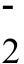
\includegraphics[width=0.8\textwidth]{assets/326}
	\caption*{}
\end{figure},
AsS\begin{figure}[H]
	\centering
	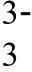
\includegraphics[width=0.8\textwidth]{assets/327}
	\caption*{}
\end{figure} and
AsS\begin{figure}[H]
	\centering
	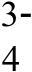
\includegraphics[width=0.8\textwidth]{assets/328}
	\caption*{}
\end{figure}, in other cases - in the form of
oxygen-containing molecules and anions. The form of existence of arsenic
in aqueous solutions depends on its valency {[}1-2{]}.

According to literature data {[}3, 4{]}, during electrorefining of
copper, 60-80\% of arsenic passes from the anode into the electrolyte,
the rest goes into sludge. The distribution of arsenic between the
electrolyte and sludge, as well as the form of its presence in the
solution, depends on the composition of the electrolyte and the
electrolysis mode. For example, the presence of As and Sb of different
valencies in the electrolyte leads to the precipitation of
antimony-arsenic (Sb\textsuperscript{3+}-As\textsuperscript{5+}) and
antimony-arsenic (Sb\textsuperscript{5+}-As\textsuperscript{3+})
precipitation. An increase in the total content of impurities in the
electrolyte leads to an increase in the electrical resistance of the
solution and its viscosity, an increase in electricity consumption, a
decrease in current efficiency and an increase in the content of harmful
impurities in the cathode metal. Therefore, blister copper, as the main
raw material of the copper electrorefining process, determines the
composition of the electrolyte during electrolysis. An increase in the
content of impurities such as nickel, arsenic and antimony leads to the
production of defective copper or copper of low grades.

During the processing of technogenic arsenic-containing materials by
hydrometallurgical methods, a large proportion of arsenic goes into
solution in trivalent form. Practice and research show that arsenic in
copper electrolyte is mainly pentavalent. For effective purification and
precipitation of sparingly soluble iron arsenates, it is necessary to
oxidize arsenic (III) ions to the pentavalent state {[}5{]}. If we take
into account that during electrochemical oxidation, metallic arsenic
forms arsenic trioxide {[}6, 7{]}, then elucidating the reasons for this
fact is an interesting problem.

The relevance of these studies is due to the need to remove arsenic from
the technological process of non-ferrous metal production in an
environmentally safe form, taking into account their subsequent storage
or disposal. Such forms are arsenates, where arsenic is pentavalent.

{\bfseries Materials and methods.} To obtain information about the behavior
of arsenic in a copper electrolyte, the chemical oxidation of As(III)
was studied in the following systems: As
(III)-H\textsubscript{2}SO\textsubscript{4}-H\textsubscript{2}O, As
(III)-MeSO\textsubscript{4}-H\textsubscript{2}O,
As(III)--H\textsubscript{2}SO\textsubscript{4}--MeSO\textsubscript{4}--H\textsubscript{2}O
(where Me - Cu, Ni, Co, Mn, Zn). Trivalent arsenic was introduced into
the studied systems in the form of sodium arsenite (0,011 gEq/l) and
solid trioxide. The influence of temperature, the amount of transition
metal ions, the duration of the experiment, and the concentration of
sulfuric acid on the degree of transition of As(III) to As(V) was
studied. Experiments were carried out with air blowing., Oxidation of
As(III) in solutions, where dissolved oxygen was previously removed by
blowing with an inert gas (argon), was also studied.

The oxidation process was carried out as follows: solutions of sulfuric
acid and transition metal sulfates were introduced into a vessel with a
NaAsO\textsubscript{2} solution, and the contents were stirred with a
magnetic stirrer for a certain time. Air and argon were supplied into
the solution under pressure while stirring.

To avoid the presence of atmospheric oxygen in the reaction zone, the
experiments were carried out under sealed conditions with constant argon
purging. Reagents for this purpose were preliminarily prepared in a box
using transition metal salts that were twice recrystallized and dried in
an argon atmosphere.

Quantitative determination of As(III) was carried out by amperometric
titration.

{\bfseries Results and discussion.} We discovered the fact of instantaneous
oxidation of As(III) in small quantities (up to 10\%) when various
amounts of sulfuric acid are added to the working solution. In this
case, the content of sulfuric acid does not change in all experiments,
i.e. the oxidation of arsenic (III) occurs with the participation of
dissolved oxygen, and the fact of the instantaneous transformation of
part of As(III) into As(V) is due to the catalytic nature of the
process. The ability of H\textsubscript{2}SO\textsubscript{4} to
increase the rate of ``spontaneous'' oxidation of arsenic in solutions
is indicated by the author of the work {[}8{]}.

The effect of catalytic oxidation of As(III) is observed in all
experiments when introducing transition metal salts into an arsenic
solution. Moreover, in As(III)-MeSO\textsubscript{4}-H\textsubscript{2}O
systems the degree of conversion reaches 25\%.

It should be noted that in the systems
As(III)-H\textsubscript{2}SO\textsubscript{4}-MeSO\textsubscript{4}-H\textsubscript{2}O
(where Me - Cu, Ni, Co, Mn, Zn), the amount of instantly oxidized
arsenic increases, and no significant dependence on the nature of the
salt (among those studied) is observed (Table 1). The degree of
transition of As(III) to As(V) depends on the concentration of metal
ions and reaches its maximum at a molar ratio of Me:As(III) above
(6\begin{figure}[H]
	\centering
	
\includegraphics[width=0.8\textwidth]{assets/329}
	\caption*{}
\end{figure}9):1.
Based on data {[}9{]} on the solubility of oxygen in aqueous solutions,
it was determined that about 60-80\% of dissolved oxygen is involved in
the process of catalytic oxidation of trivalent arsenic.

The duration of the process and temperature do not play a significant
role. This is evidenced by the following experimental data: within 6
hours after instant oxidation, the transition of As(III) to As(V) in the
As(III)-H\textsubscript{2}SO\textsubscript{4}-H\textsubscript{2}O system
was about 6-7\%, and in a solution, for example, containing 0,1 gEq/l of
copper sulfate, the degree of conversion at temperatures of
22\textsuperscript{0}C, 40\textsuperscript{0}C and
60\textsuperscript{0}C was 34.5\%, 34.8\% and 36\%, respectively. The
results of experiments on the oxidation of As(III) in the presence of
ions of other transition metals under study are relatively close to
these data.

{\bfseries Table 1 - The degree of conversion of As(III) (\%) in a sulfuric
acid medium in the presence of transition metal ions and an adsorbing
surface (Pt plate) when blown with air}

{\bfseries (C}\begin{figure}[H]
	\centering
	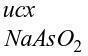
\includegraphics[width=0.8\textwidth]{assets/330}
	\caption*{}
\end{figure} {\bfseries = 0,011 gEq/l,
C}\begin{figure}[H]
	\centering
	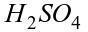
\includegraphics[width=0.8\textwidth]{assets/331}
	\caption*{}
\end{figure} {\bfseries = 0,12 gEq/l, t =
60\textsuperscript{0}C, τ = 3 hours)}

% \begin{longtable}[]{@{}
%   >{\raggedright\arraybackslash}p{(\columnwidth - 6\tabcolsep) * \real{0.0794}}
%   >{\raggedright\arraybackslash}p{(\columnwidth - 6\tabcolsep) * \real{0.2698}}
%   >{\raggedright\arraybackslash}p{(\columnwidth - 6\tabcolsep) * \real{0.3333}}
%   >{\raggedright\arraybackslash}p{(\columnwidth - 6\tabcolsep) * \real{0.3174}}@{}}
% \toprule\noalign{}
% \endhead
% \bottomrule\noalign{}
% \endlastfoot
% Ме & Concentration
% 
% C\begin{figure}[H]
% 	\centering
% 	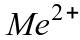
\includegraphics[width=0.8\textwidth]{assets/332}
% 	\caption*{}
% \end{figure} ⋅ 10\textsuperscript{-2} gEq/l &
% Effect of catalytic oxidation, \% & Oxidation state of As(III) in the
% presence of the ion
% 
% Me\textsuperscript{2+}, \% \\
% - & - & 4,21 & 29,0 \\
% \multirow{3}{=}{Cu} & 4,8 & 21,4 & 51,9 \\
% & 7,8 & 33,5 & 60,2 \\
% & 9,8 & 33,8 & 60,1 \\
% \multirow{3}{=}{Ni} & 4,8 & 32,9 & 49,4 \\
% & 7,8 & 34,9 & 58,2 \\
% & 9,8 & 34,9 & 57,7 \\
% \multirow{3}{=}{Co} & 4,8 & 33,6 & 54,1 \\
% & 7,8 & 31,7 & 58,6 \\
% & 9,8 & 32,1 & 58,7 \\
% \multirow{3}{=}{Mn} & 4,8 & 30,0 & 52,5 \\
% & 7,8 & 30,8 & 55,3 \\
% & 9,8 & 30,0 & 55,0 \\
% \multirow{3}{=}{Zn} & 4,8 & 33,9 & 50,8 \\
% & 7,8 & 34,8 & 55,2 \\
% & 9,8 & 30,5 & 54,9 \\
% \end{longtable}

Our experiments have shown that blowing air through solutions has such a
weak effect on the oxidation process in the systems under study that
even for 3 or more hours, air bubbling both in the
As(III)-H\textsubscript{2}SO\textsubscript{4}-H\textsubscript{2}O system
and in the system
As(III)-H\textsubscript{2}SO\textsubscript{4}-MeSO\textsubscript{4}-H\textsubscript{2}O
did not lead to significant oxidation of As(III). Varying the
temperature in the range of 20-60\textsuperscript{0}C did not have a
significant effect on the progress of the process.

In experiments with air blowing, the oxidation process of As(III) can be
intensified at the liquid-solid interface due to the sorption of oxygen
on it. In addition, the interface is an integral element of the copper
electrorefining process, which to some extent brings the experimental
conditions closer to production ones. We tested the effect of a platinum
plate immersed in the reaction zone on the oxidation of As(III). This
metal has the ability to adsorb oxygen on its surface and oxidation on
such a surface occurs with the participation of oxygen from platinum
oxides {[}10{]}, according to the scheme:

AsO\begin{figure}[H]
	\centering
	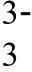
\includegraphics[width=0.8\textwidth]{assets/333}
	\caption*{}
\end{figure} + PtO{[}O{]}
\begin{figure}[H]
	\centering
	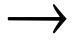
\includegraphics[width=0.8\textwidth]{assets/334}
	\caption*{}
\end{figure}
AsO\begin{figure}[H]
	\centering
	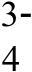
\includegraphics[width=0.8\textwidth]{assets/335}
	\caption*{}
\end{figure} + PtO

Initially, the
As(III)-H\textsubscript{2}SO\textsubscript{4}-H\textsubscript{2}O system
was studied with air blowing in the presence of a Pt plate. At the same
time, at the initial moment, the oxidation of As(III) is a fairly
intense process, which slows down over time. Thus, at a temperature of
21\textsuperscript{0}C in 2 hours the degree of conversion was 26,7\%,
and in the next 1,5 hours it increased by only 2\%. Increasing the
temperature of the working solution to 60\textsuperscript{0}C allowed us
to speed up the process. In this case, the same amount of As(III) -
26.7\% transforms into As(V) in 0,5 hours, and subsequent oxidation
takes a long time.

Another factor that had a significant impact on the oxidation of As(III)
in the presence of a Pt plate was the introduction of transition metal
ions (Cu, Ni, Co, Mn, Zn) into the working solution, the ability of
which to reversibly bind and activate oxygen is well known {[}11{]}. The
highest degree of transition of As(III) to As(V) was recorded at a
temperature of 60\textsuperscript{0}C. Within 3 hours, the percentage of
conversion of trivalent arsenic reaches 55-60\%, where the effect of
catalytic oxidation is about 30-35\%. These results (Table 1) are
further evidence of the participation of atmospheric oxygen in the
process of catalytic oxidation of As(III) in the presence of some
transition metal ions. The importance of iron, copper and zinc ions in
the oxidation of arsenic was also confirmed in works {[}12-14{]}.

Therefore, if the presence of oxygen in the reaction zone is eliminated,
the oxidation of As(III) should be practically absent. For this purpose,
we conducted experiments with preliminary blowing of argon through a
NaAsO\textsubscript{2} solution and a sulfuric acid solution of
MeSO\textsubscript{4} (where Me is Cu, Ni, Co, Mn, Zn) before mixing
them. The experiments were carried out at a temperature of
60\textsuperscript{0}C and constant bubbling with argon with stirring.
Within 3 hours, we observed a slight decrease in the concentration of
As(III), which was about 5\%. In our opinion, the observed phenomenon is
explained by the fact that blowing argon does not contribute to the
complete removal of oxygen bound in the active complex. In our opinion,
the activation of oxygen by transition metal ions occurs in the process
of hydrolysis of these ions and complex formation. Thus, in an aqueous
solution of CuSO\textsubscript{4}, hydrated ions
{[}Cu(H\textsubscript{2}O)\textsubscript{4}{]}\textsuperscript{2+} are
able to attach an oxygen molecule O\textsubscript{2} as a weak ligand,
promoting its activation. Based on this, solutions of sulfuric acid and
transition metal salts were prepared in an inert environment-box. Purge
of trivalent arsenic solution with argon began 0,5 hour before mixing
the solutions and was carried out throughout the experiment. Under the
conditions of this experiment, the percentage of oxidation was 0,5\%
within 3 hours. Those. Despite a slight decrease in the degree of
As(III) conversion under these conditions, we were not able to
completely eliminate the presence of oxygen in the system.

The catalytic role of transition metal ions in the oxidation of arsenic
is also evidenced by the results of our studies of the behavior of solid
arsenic trioxide in sulfuric acid solutions in the presence of
Cu\textsuperscript{2+}, Ni\textsuperscript{2+}, Co\textsuperscript{2+},
Mn\textsuperscript{2+}, Zn\textsuperscript{2+} ions (Table 2). The
dissolution of As\textsubscript{2}O\textsubscript{3} in sulfuric acid
solutions is a slow process with simultaneous oxidation of
As\textsuperscript{3+} to As\textsuperscript{5+} in the liquid phase. As
can be seen from Table 2, the influence of transition metal ions on the
oxidation of solid arsenic trioxide is very significant. The degree of
transition of As\textsuperscript{3+} to As\textsuperscript{5+} increases
with increasing temperature of the reaction mixture.

{\bfseries Table 2 - Degree of conversion of
As\textsubscript{2}O\textsubscript{3} (\%) in a sulfuric acid medium in
the presence of transition metal ions (Me\textsuperscript{2+})
(m}\begin{figure}[H]
	\centering
	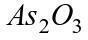
\includegraphics[width=0.8\textwidth]{assets/336}
	\caption*{}
\end{figure}{\bfseries = 0,30 g,
C}\begin{figure}[H]
	\centering
	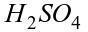
\includegraphics[width=0.8\textwidth]{assets/331}
	\caption*{}
\end{figure}{\bfseries = 0,12 gEq/l,
C\emph{\textsubscript{Me2+}} = 0,10 gEq/l,}

{\bfseries V = 50 ml, τ = 3 hours) depending on the temperature when
blowing air}

\begin{longtable}[]{@{}
  >{\raggedright\arraybackslash}p{(\columnwidth - 12\tabcolsep) * \real{0.2032}}
  >{\raggedright\arraybackslash}p{(\columnwidth - 12\tabcolsep) * \real{0.1250}}
  >{\raggedright\arraybackslash}p{(\columnwidth - 12\tabcolsep) * \real{0.1250}}
  >{\raggedright\arraybackslash}p{(\columnwidth - 12\tabcolsep) * \real{0.1250}}
  >{\raggedright\arraybackslash}p{(\columnwidth - 12\tabcolsep) * \real{0.1250}}
  >{\raggedright\arraybackslash}p{(\columnwidth - 12\tabcolsep) * \real{0.1407}}
  >{\raggedright\arraybackslash}p{(\columnwidth - 12\tabcolsep) * \real{0.1562}}@{}}
\toprule\noalign{}
\endhead
\bottomrule\noalign{}
\endlastfoot
Temperature, \textsuperscript{о}С &
\multicolumn{6}{>{\raggedright\arraybackslash}p{(\columnwidth - 12\tabcolsep) * \real{0.7968} + 10\tabcolsep}@{}} \\
& - & Сu\textsuperscript{2+} & Ni\textsuperscript{2+} &
Co\textsuperscript{2+} & Mn\textsuperscript{2+} &
Zn\textsuperscript{2+} \\
20 & 0,040 & 14,9 & 13,6 & 14,1 & 13,5 & 12,8 \\
40 & 0,084 & 26,4 & 23,0 & 24,9 & 24,8 & 21,1 \\
60 & 0,120 & 58,2 & 54,9 & 56,4 & 56,0 & 52,1 \\
\end{longtable}

{\bfseries Conclusions.} Thus, the stage of the transition of arsenic from
the trivalent to the pentavalent state occurs with the participation of
atmospheric oxygen and occupies a central place in the process of anodic
oxidation of elemental arsenic in sulfuric acid solutions in the
presence of Cu\textsuperscript{2+}, Ni\textsuperscript{2+},
Co\textsuperscript{2+}, Mn\textsuperscript{2+}, Zn\textsuperscript{2+}
ions, and the nature of the studied transition metal salts does not have
a significant effect on the degree of As(III) conversion. This property
of some transition metal ions to catalytically oxidize As(III) was used
by us later in the development of new methods for processing copper
electrolyte with transition metal compounds with the removal of arsenic
in the form of arsenates. In practice, preliminary introduction of
transition metals into arsenic-containing solutions will allow the
arsenic to be maximally converted into the pentavalent state, which will
ensure their effective purification with the removal of arsenic in an
environmentally safe form.

{\bfseries References}

1. Tolstikov V. P. Vzaimozavisimost\textquotesingle{}
okislitel\textquotesingle no-vosstanovitel\textquotesingle nyh processov
i pH reakcionnoj sredy // Zhurnal obshhej himii. - 1969. -Vyp. 39, -№ 2.
-S. 240-247. {[}in Russian{]}

2. Levin A.I., Nomberg M.I. Jelektroliticheskoe rafinirovanie medi. --
M.: Metallurgizdat, 1963. -219 s. {[}in Russian{]}

3. Bajmakov Ju. V., Zhurin A. I. Jelektroliz v gidrometallurgii. -- M.:
Metallurgija, 1977. -336 s. {[}in Russian{]}

4. Kuznecova T. A., Fedorov V.A. Jelektroliticheskoe rafinirovanie medi
s povyshennym soderzhaniem Sb i As i vyvod ih iz jelektrolita //
Metallurgija cvetnyh metallov. -1974.-№ 4. -S. 174-179. {[}in Russian{]}

5. Tret\textquotesingle jak M.A., Karimov K.A., Nabojchenko S.S.
Avtoklavnoe okislenie ionov mysh\textquotesingle jaka (III) ionami
zheleza (II), (III) // Sovremennye tehnologii proizvodstva cvetnyh
metallov : materialy Mezhdunarodnoj nauchnoj konferencii, posvjashhennoj
80-letiju S. S. Nabojchenko, Ekaterinburg, 24--25 marta 2022 g. -
Ekaterinburg: Izdatel\textquotesingle stvo Ural\textquotesingle skogo
universiteta, 2022. - S. 68-72. http://elar.urfu.ru/handle/10995/110239.
{[}in Russian{]}.

6. Efimov E. A., Erusalimchik I. G. Jelektrohimicheskie processy na
mysh\textquotesingle jakovom jelektrode // Jelektrohimija. -1965. -Vyp.
1, -№ 9. -S. 1133- 1137. {[}in Russian{]}

7. Tomilov A. P., Osadchenko I. M., Homutov E. M. Jelektrohimija
mysh\textquotesingle jaka i ego soedinenij. Itogi nauki i tehniki VINITI
AN SSSR // Jelektrohimija. -1979. -№ 14. -S. 168-207. {[}in Russian{]}

8. Uil\textquotesingle jams U.Dzh. Opredelenie anionov. -M.:
Himija,Spravochnik. Per. s angl. --- M.: Himija, 1982 --- 624 s. {[}in
Russian{]}

9. Rabinovich V.A., Havin Z.Ja. Kratkij himicheskij spravochnik.
-Leningrad: Himija, 1978. -392 s. ISBN: 5-7245-0703-X. {[}in Russian{]}

10. Kasenov B.K., Aldabergenov M.K., Pashinkin A.S. Termodinamicheskie
metody v himii i metallurgii. Almaty: Rauan, 1994. -126 s. ISBN
5-625-02445-6. {[}in Russian{]}

11. Basolo F., Pirson R. Mehanizmy neorganicheskih reakcij. M.: Mir,
1971. -592 s. {[}in Russian{]}

12. Perelomov L.V., Perelomova I.V., Levkin N.D. i dr. Adsorbcija i
okislenie soedinenij mysh\textquotesingle jaka mineralami zheleza i v
bio-mineral\textquotesingle nyh sistemah // Izvestija
Tul\textquotesingle skogo gosudarstvennogo universiteta. Estestvennye
nauki. -2012. -Vyp. 3. -S. 231-241. {[}in Russian{]}

13. K.Z. Song, P. C Ke, Z. Y. Liu et. аl. Co-oxidation of arsenic (III)
and iron (II) ions by pressurized oxygen in acidic solutions / // Int.
J. Miner. Metall. Mater. - 2020. - № 27. - Р. 181-189.
https://dx.doi.org/10.1007/s12613-019-1786-9

14. P. Zhang, C. Li, C. Wei et. аl. Effects of zinc and copper ions on
ferric arsenate precipitation in hydrothermal scorodite // J. Cent.
South Univ. Sci. Technol. - 2019. - № 50. - Р. 2645--2655.

\emph{{\bfseries Information about authors}}

Omarov K.B. - Doctor of Technical Sciences, Professor, Kazakh University
of Technology and Business named after K.Kulazhanov, Astana, Kazakhstan,
e-mail: homarov1963@mail.ru;

Nurtai Zh.T. - PhD, Associate Professor, Kazakh University of Technology
and Business named after K.Kulazhanov, Astana, Kazakhstan, e-mail:
zhadira\_nurtai@mail.ru;

Nurgaliyev N.U. - Candidate of Chemical Sciences, Associate Professor,
Kazakh University of Technology and Business, Astana,, Kazakhstan named
after K.Kulazhanov, e-mail: nurgaliev\_nao@mail.ru;

Takirova A.K. - master\textquotesingle s degree, senior lecturer, Kazakh
University of Technology and Business named after K. Kulazhanov, Astana,
Kazakhstan, e-mail: adem\_1996@mail.ru

\emph{{\bfseries Сведения об авторах}}

Омаров Х.Б. - доктор технических наук, профессор, профессор, Казахский
университетт технологии и бизнеса имени К.Кулажанова, Астана, Казахстан,
e-mail: homarov1963@mail.ru;

Нұртай Ж.Т. - доктор PhD, ассоциированный профессор, Казахский
университет технологии и бизнеса имени К.Кулажанова, Астана Казахстан, ,
e-mail: zhadira\_nurtai@mail.ru;

Нургалиев Н.У. - кандидат химических наук, доцент, Казахский университет
технологии и бизнеса имени К.Кулажанова, Республика Казахстан, Астана,
e-mail: nurgaliev\_nao@mail.ru;

Такирова A.Х. - магистр, старший преподаватель, Казахский университет
технологии и бизнеса имени К.Кулажанова, Республика Казахстан, Астана,
e-mail: аdem\_1996@mail.ru\newpage
{\bfseries IRSTI 53.01.91}

{\bfseries PROCESSING OF SOLID ARSENIC -CONTAINING MATERIALS}

(analytical review)

{\bfseries \textsuperscript{1}N.I. Kopylov,
\textsuperscript{2}Kh.B.Omarov\textsuperscript{🖂}}

\textsuperscript{1}Institute of Solid State Chemistry and
Mechanochemistry, Siberian Branch Russian Academy of Sciences,
Novosibirsk, Russia,

\textsuperscript{2} K.Kulazhanov named Kazakh University of Technology
and Business, Astana, Kazakhstan

{\bfseries \textsuperscript{🖂}}Correspondent-author: homarov1963@mail.ru

This article provides an analytical review of scientific and technical
developments in the processing of solid arsenic-containing materials.
Hydro-, pyrometallurgical and combined methods for extracting arsenic
from dust, sublimates, and sludge from metallurgical production are
considered. The most acceptable technologies seem to be those in which
arsenic is removed from the process at the preliminary stage of
processing in the most stable, non-toxic form - arsenic sulfides, which
exist in nature as orpiment and realgar minerals. Studies conducted at
the Zh. Abishev Chemical and Metallurgical Institute (Karaganda,
Republic of Kazakhstan) and the Gidrotsvetmet Institute (Novosibirsk,
Russian Federation) on products from a number of arsenic-containing raw
material deposits for the removal of arsenic by oxidizing-sulfidizing
roasting in a shaft-type furnace have shown the promise of this
technology. The removal of arsenic from roasting products was 97-98.5\%,
simultaneously with the production of compact sulfide material with an
arsenic content of 60-70\% that does not require special disposal.

{\bfseries Key words:} metallurgical production, arsenic-containing
materials, leaching, oxidation-sulfiding roasting, acid, autoclave,
bacterial oxidation, arsenates, oxides and sulfides of arsenic.

{\bfseries ҚҰРАМЫНДА МЫШЬЯК БАР ҚАТТЫ МАТЕРИАЛДАРДЫ ӨҢДЕУ}

(аналитикалық шолу)

{\bfseries \textsuperscript{1}Н.И. Копылов,
\textsuperscript{2}Х.Б.Омаров\textsuperscript{🖂}}

\textsuperscript{1}Қатты денелер химиясы және механикохимия институты,
Сібір бөлімшесі Ресей ғылым академиясы, Новосибирск, Ресей,

\textsuperscript{2} Қ.Құлажанов атындағы Қазақ технология және бизнес
университеті, Астана, Қазақстан,

e-mail: homarov1963@mail.ru

Бұл мақалада мышьяк бар қатты материалдарды өңдеудегі ғылыми-техникалық
әзірлемелерге аналитикалық шолу берілген. Металлургиялық өндірістегі
шаңдардан, сублиматтардан және шламдардан мышьяк алудың гидро-,
пирометаллургиялық және аралас әдістері қарастырылған. Табиғатта
аурипигмент және реальгар минералдары түрінде болатын мышьяк сульфидтері
- мышьяк ең тұрақты, улы емес түрінде өңдеудің алдын ала сатысында
процестен шығарылатын технологиялар ең қолайлы болып табылады. Әбішев
атындағы Химия-металлургия институтында (Қарағанды, Қазақстан
Республикасы) және Гидроцветмет институтында (Новосибирск, Ресей
Федерациясы) мышьякты жою бойынша бірқатар кен орындарының өнімдеріне
жүргізілген зерттеулер. шахталық пеште тотықтырғыш-сульфидтендіргіш
күйдіру осы технологияның болашағын көрсетті. Қуырылған өнімдерден
мышьякты кетіру 97-98,5\% құрады, арнайы көмуді қажет етпейтін мышьяк
мөлшері 60-70\% болатын ықшам сульфидті материалды алумен бір мезгілде.

{\bfseries Түйін сөздер:} металлургиялық өндіріс, құрамында мышьяк бар
материалдар, сілтілеу, тотықтырғыш-сульфидтендіргіш күйдіру, қышқыл,
автоклав, бактериялық тотығу, арсенаттар, мышьяк оксидтері және
сульфидтер.

{\bfseries ПЕРЕРАБОТКА ТВЕРДЫХ МЫШЬЯКСОДЕРЖАЩИХ МАТЕРИАЛОВ}

(аналитический обзор)

{\bfseries \textsuperscript{1} Н.И. Копылов,
\textsuperscript{2}Х.Б.Омаров\textsuperscript{🖂 }}

Институт химии твердого тела и механохимии Сибирского отделения

Российской Академии наук, Новосибирск, Россия,

Казахский университет технологии и бизнеса имени К.Кулажанова, Астана,
Казахстан,

e-mail: homarov1963@mail.ru

В данной статье приведен аналитический обзор научно-технических
раработок по переработке твердых мышьяксодержащих материалов.
Рассмотрены гидро-, пирометаллургические и комбинированные методы
извлечения мыщьяка из пылей, возгонов, шламов металлургического
производства. Наиболее приемлемыми представляются технологии, по которым
мышьяк на предварительной стадии передела выводится из процесса в
наиболее устойчивой, нетоксичной форме -- сульфидов мышьяка,
существующих в природе в виде минералов аурипигмента и реальгара.
Исследования, проведенные в Химико-металлургическом институте имени
Ж.Абишева (г. Караганда, Республика Казахстан) и институте
«Гидроцветмет» (г. Новосибирск, Российская Федерация) на продуктах
целого ряда месторождений мышьяксодержащего сырья по выводу мышьяка
окислительно-сульфидизирующим обжигом в печи шахтного типа, показали
перспективность данной технологии. Вывод мышьяка из продуктов обжига
составил 97-98,5 \%, одновременно с получением компактного, не
требующего специального захоронения сульфидного материала с содержанием
мышьяка 60-70\%.

{\bfseries Ключевые слова:} металлургическое производство, мышьяксодержащие
материалы, выщелачивание, окислительно-сульфидизирующий обжиг,
кислотное, автоклавное, бактериальное окисление, арсенаты, оксиды и
сульфиды мышьяка.

{\bfseries Introduction.} One of the problematic objects in the production
of heavy non-ferrous metals is arsenic, which is present in various
concentrations in ores and concentrates of non-ferrous and noble metals.
During their processing, arsenic leads to various technological
difficulties that worsen the quality of the base metal and other
by-products. The process is accompanied by environmental pollution with
arsenic, its accumulation in intermediate products, mandatory
neutralization and storage of arsenic-containing materials.

Metallurgical arsenic-containing industrial objects are conventionally
classified into four classes:

- natural raw materials, where arsenic phases are represented by
arsenopyrite, iron arsenides, thioarsenates and arsenides of non-ferrous
metals;

- products of metallurgical oxidation processes, where the form of
arsenic is arsenates, its oxides;

- products of reduction processes, where arsenic is elemental,
arsenides;

- sulfur and phosphorus (chalcogenides) of technical grades, where
arsenic is in the form of sulfides and monophosphide.

Products of arsenic purification of gases (dust, sublimes) and waste
water (cakes, sediments) in addition to arsenic contain significant
amounts of other valuable metals, as shown in Table 1.

The disposal of these materials is a complex technical problem and
includes either their comprehensive processing or safe disposal. The
degree of arsenic sublimation is determined by the composition and
temperature of the slag and matte, the temperature and composition of
the exhaust gases, as well as the partial pressure of oxygen in the gas
phase and a number of other factors {[}1, 2{]}. Most of the arsenic in
the dusts is in the form of arsenates (70\%), approximately 15\% of the
total content is oxides. The zinc and lead content reaches 9.7 and
36.8\%, respectively.

During the processing of copper raw materials and copper-containing
semi-finished products of lead production, lead, arsenic and other
metals are concentrated in converter dusts. Up to 90\% of lead, more
than 90\% of arsenic, up to 95\% of cadmium and more than 65\% of
rhenium and selenium from the amounts contained in the matte pass into
them. Fine converter dusts contain, \%: 42-50 lead, 0.3-0.7 cadmium,
15-28 arsenic, 0.3-0.5 bismuth, 0.2-1.0 selenium and 30-70 g / t
rhenium. The transfer of these dusts to lead production is one of the
main factors in the intra- and inter-plant circulation of arsenic.

{\bfseries Table 1-Chemical composition of dust and sublimates from
metallurgical production, \%}

\begin{longtable}[]{@{}
  >{\raggedright\arraybackslash}p{(\columnwidth - 14\tabcolsep) * \real{0.4698}}
  >{\raggedright\arraybackslash}p{(\columnwidth - 14\tabcolsep) * \real{0.0758}}
  >{\raggedright\arraybackslash}p{(\columnwidth - 14\tabcolsep) * \real{0.0759}}
  >{\raggedright\arraybackslash}p{(\columnwidth - 14\tabcolsep) * \real{0.0759}}
  >{\raggedright\arraybackslash}p{(\columnwidth - 14\tabcolsep) * \real{0.0759}}
  >{\raggedright\arraybackslash}p{(\columnwidth - 14\tabcolsep) * \real{0.0758}}
  >{\raggedright\arraybackslash}p{(\columnwidth - 14\tabcolsep) * \real{0.0759}}
  >{\raggedright\arraybackslash}p{(\columnwidth - 14\tabcolsep) * \real{0.0752}}@{}}
\toprule\noalign{}
\begin{minipage}[b]{\linewidth}\raggedright
Arsenic containing materials
\end{minipage} & \begin{minipage}[b]{\linewidth}\raggedright
As
\end{minipage} & \begin{minipage}[b]{\linewidth}\raggedright
Sn
\end{minipage} & \begin{minipage}[b]{\linewidth}\raggedright
Pb
\end{minipage} & \begin{minipage}[b]{\linewidth}\raggedright
Zn
\end{minipage} & \begin{minipage}[b]{\linewidth}\raggedright
Cu
\end{minipage} & \begin{minipage}[b]{\linewidth}\raggedright
Fe
\end{minipage} & \begin{minipage}[b]{\linewidth}\raggedright
S
\end{minipage} \\
\midrule\noalign{}
\endhead
\bottomrule\noalign{}
\endlastfoot
Fuming sublimates of tin production

1.

2.

3. & 7,4

1,6

2,4 & 40,8

13,2

66,2 & 13,8

11,7

0,4 & 4,1

47,8

2,7 & 0,05

0,17

0,03 & 0,5

-

- & 3,7

4,5

0,8 \\
Fuming sublimates of lead-zinc production & 0,92 & - & 12,2 & 58,6 &
0,75 & 0,6 & 1.4 \\
Dust from electric smelting of tin raw materials & 1,1 & 27,6 & 1,2 &
28,4 & 0,03 & - & 1,1 \\
Polymetallic raw material electric smelting dust & 2,7 & 12,6 & 14,5 &
34,6 & 0,13 & - & 5,0 \\
Electric smelting dust from tin refining & 1,5 & 34,2 & 0,2 & 0,8 & 0,16
& - & 0,4 \\
Electric smelting dust from refining of Pb-Sn alloys & 2,6 & 18,5 & 27,4
& 6,9 & 1,5 & 0,4 & 2,5 \\
Dust from agglomeration and shaft smelting of lead concentrates & 5,1 &
- & 54,8 & 11,8 & 0,22 & - & - \\
Dust from roasting zinc concentrates & 2,1 & - & 31,7 & 14,0 & 0,74 &
2,1 & 13,6 \\
Dust from the smelting of copper sulphide concentrates & 1,0 & - & 8,3 &
7,0 & 13,0 & 5,4 & 28,5 \\
Copper production converter dust & 5,9 & - & 32,2 & 18,9 & 3,3 & - &
- \\
\end{longtable}

Copper-containing cakes are mainly added to the smelting furnace charge.
This is the simplest and least expensive method, but it seems the least
rational, since arsenic is returned to the copper smelting production,
accumulates in the electrolyte, thereby worsening the indicators and
ecology of the process.

The variety of methods for processing arsenic-containing dusts,
sublimates, and sludge from metallurgical production can be
conditionally divided into hydro-, pyrometallurgical, and combined
methods.

\emph{Hydrometallurgical methods.} A large set of reagents has been
proposed for extracting arsenic from dusts and sublimates: sulfuric,
hydrochloric and nitric acids, solutions of sodium and ammonium
carbonates, caustic soda, sodium sulfide and others. However, most of
them are not selective: heavy non-ferrous metals also pass into the
solution, which complicates their subsequent processing {[}1{]}.
Nevertheless, there are developments that meet the conditions of
selectivity.

For example, in work {[}2{]}, arsenic from arsenic-containing materials
was transferred into a solution with sodium hydroxide or sulfide.
Experiments have shown that under optimal conditions, the degree of
arsenic extraction into the solution in both cases reaches 95-98\%. In
the case of materials containing arsenic in the form of oxides, good
results are achieved using hot water leaching. Extraction from tin
production roasting furnace dust (44\%
As\textsubscript{2}O\textsubscript{3}) into solution is 93\% As.
Satisfactory selectivity of arsenic extraction (88-93\%) is achieved by
leaching converter dust from lead production with sodium sulfide
solutions (concentration 80-100 g/dm\textsuperscript{3}, 90-95
\textsuperscript{0}C, L:S = 6:1, 1 h). With three-stage leaching,
arsenic extraction reaches 99\%.

Selective extraction of arsenic into an alkaline solution can be
achieved by electrolytic leaching of dusts. Optimum process conditions:
С\textsubscript{NaOH} = 90-100 g/dm\textsuperscript{3}, L:S = (3-4):1.5,
50-75 \textsuperscript{0}C, D\textsubscript{k} = 1000-3000
A/cm\textsuperscript{2}. Lead is released at the cathode in the form of
a spongy sediment. To bind and precipitate lead and zinc from the
solution during leaching of arsenic with strong hot solutions of caustic
soda (100-250 g/dm\textsuperscript{3}), an additional 10-20
g/dm\textsuperscript{3} of sodium sulfide is added to the alkaline
solution {[}3{]}.

It is proposed to leach copper smelting converter dusts with 1.3-5.0\%
As and high contents of non-ferrous metals with sodium sulfide and
precipitate arsenic with various reagents, such as calcium oxide, copper
or iron sulfate, a mixture of phosphoric acid with calcium hydroxide
{[}4-6{]}. The scheme provides for the possibility of further processing
of sediments to obtain antiseptics for wood preservation or their safe
storage. When processing converter dusts with sodium sulfide solutions
(80 g / dm\textsuperscript{3} Na\textsubscript{2}S, 90
\textsuperscript{0}C, L:S = 1:6), 92.9\% of arsenic was extracted into
the solution in the form of thiosalt after 1 hour. With three-stage
leaching - up to 99\%.

For selective and deep (92-96\%) extraction of arsenic from tin
production fuming sublimates, alkaline leaching at a NaOH concentration
of 100-150 g/dm\textsuperscript{3}, L:S = 1:5-10, 80-100
\textsuperscript{0}C, duration of 1-2 h, stoichiometric
Na\textsubscript{2}S consumption for binding lead and zinc into sulfides
is proposed.

The most common method for extracting arsenic from copper-containing
cakes is the alkaline leaching scheme and subsequent precipitation of
calcium arsenate. The cake is treated with an alkali solution (70-90
g/dm\textsuperscript{3} NaOH) at 70-90 \textsuperscript{0}C, a
solid:liquid ratio of 5, and a time of 1-3 hours. Extraction into the
solution is 90-98\% As and no more than 1.0-1.5\% Cu. The
copper-containing residue can be returned to the batch preparation
department of the smelting shop. By introducing lime pulp (with a CaO:As
ratio \textgreater{} 1.5) into the solution at 80-90
\textsuperscript{0}C in 1.5-3 hours, it is possible to precipitate a
product containing 90-96\% As. This achieves alkali regeneration, and
the filtrate is returned to the alkaline leaching stage. As a result,
more than 90-92\% of arsenic passes into the burial product, and the
alkali consumption, taking into account regeneration, is 0.05 kg/kg As.

To extract copper and arsenic from copper electrolyte production
middlings, copper-arsenic cake is leached at a mass ratio of
H\textsubscript{2}SO\textsubscript{4}/Cu = (1.53-1.54):1. The leaching
solution is cooled to 20-80 \textsuperscript{0}C, the copper-containing
product is isolated, which is returned to the main production. The
mother liquor is evaporated to an As concentration of 600-800
g/dm\textsuperscript{3} and used to prepare antiseptic compositions.

Complex processing of lead production dust is complicated by its high
content of harmful impurities. The method of granulation with strong
sulfuric acid and subsequent heat treatment of the resulting granules in
a FB (fluidized bed) furnace allows removing up to 80-85\% of arsenic in
the "head" of the process and then extracting valuable components from
the resulting product {[}7{]}. Sublimates are captured in a wet gas
cleaning system, where the arsenic content in the solution reaches 20-30
g/dm\textsuperscript{3}, and in the sludge up to 40\%. The sludge is
leached and arsenic is precipitated from the combined solution with lime
milk in the form of calcium arsenate (10-12\% As).

There are developments of autoclave technologies for extracting arsenic
from dusts from processing copper and lead concentrates. Depending on
the composition of the dusts, solutions of sulfuric, nitric or
hydrochloric acids and a number of other reagents are used for their
leaching and removal of arsenic.

The process of arsenic dissolution in an alkaline solution can be
combined with the electrolytic extraction of heavy non-ferrous metals on
the cathode. In this case, alkali regeneration occurs, due to which the
equilibrium in the system shifts towards arsenic dissolution.
Alkaline-electrolytic treatment of converter dust ensures almost
complete extraction of arsenic (96-98\%) into the solution and lead
(91\%) into the cathode sponge. Zinc, cadmium, mercury, tellurium are
concentrated in an insoluble precipitate. In this case, there is a risk
of arsine formation. To prevent this during electrolysis, the original
dust is pre-treated with a 4\% NaOH solution. The alkaline solution
containing arsenic is fortified with alkali to 120
g/dm\textsuperscript{3}, cooled to 18-20 \textsuperscript{0}C and, after
separating the sodium arsenate crystals, sent for leaching of a new
portion of dust. Sodium arsenate is dissolved in water at 60-70
\textsuperscript{0}C and calcium arsenate is precipitated from the
resulting solution (50-60 g/dm\textsuperscript{3} As) with lime milk,
which is sent for disposal {[}3{]}.

\emph{Pyrometallurgical and combined methods.} At non-ferrous metallurgy
plants, up to 30\% of arsenic is concentrated in dust and sublimates
{[}8, 9{]}.

When processing sulfide copper concentrates with a low arsenic content
(up to 1\%) in order to obtain arsenic-free gases during smelting, it
was proposed {[}10{]} to roast the concentrate at 750
\textsuperscript{0}C in a mixture with calcium hydroxide in an amount
from 1.5 to 3 times greater than the stoichiometric amount required to
bind arsenic into calcium arsenate. During subsequent smelting, the
resulting calcium arsenate is converted into waste slag.

For relatively arsenic-rich materials (\textgreater5\% As) that do not
contain other subliming components, the main part of the arsenic
(80-90\%) can be distilled off in the form of sublimates containing up
to 90-98\% As\textsubscript{2}O\textsubscript{3} by firing at 550-700
\textsuperscript{0}C in multiple-hearth, muffle or other furnaces. In
order to prevent the formation of higher arsenic oxides and accelerate
the distillation, up to 10\% of fine coal and a sulfidizer (pyrite) are
added to the batch {[}11{]}. Metallurgical sublimates and dusts are
subjected to various types of smelting with concentration of valuable
metals (lead, zinc and others) in the melt, and arsenic - in sublimates
or in melts of rough alloy, mattes, slags. Sodium hydroxide, soda,
sodium sulfate, their mixtures are used as slag- and matte-forming
fluxing components. The process is carried out in a controlled
environment with the introduction of coke into the charge.

When smelting dusts using only sodium sulfate (22-30\% of the dust
mass), 75\% of the arsenic passes into the matte-slag melt and 23\% into
the crude lead. 93\% of the lead is concentrated in the lead melt. When
using a mixture of sodium sulfate and soda (40-45\% of the mixture in
the charge), the arsenic is concentrated in the matte-slag melt, and
with an excess of soda (about 60\%), 75-80\% of the arsenic passes into
the crude lead and only 20\% into the matte-slag melt. The extraction of
lead into the melt, containing 9.3\% As, was 93-94\% of the content in
the original dust. As a result, arsenic can be concentrated in either
the crude lead or the matte-slag melt during the smelting process, if
necessary. Black lead with a high arsenic content can be suitable for
special alloys for various purposes (high-capacity batteries, bearings,
etc.). Arsenic is leached from the stein-slag melt with water and then
precipitated with lime.

Systematic research and technological developments on the removal of
arsenic from metallurgical processes in the form of a non-toxic,
storable product -- sulfide -- were carried out at the Zh. Abishev
Chemical and Metallurgical Institute (Karaganda) {[}12-16{]}. A method
was developed for obtaining arsenic sulfide sublimates from sulfide
materials by roasting them at 650-700 \textsuperscript{0}C in a mixture
with pyrite in a ratio of arsenic to arsenic in the charge equal to
(1.8-2):1, followed by melting the powdered sublimates and obtaining a
compact alloy that is not oxidized in air and insoluble in water.
Methods have also been proposed for converting arsenic dust into sulfide
by sulfiding it with elemental sulfur at a temperature of 325-350
\textsuperscript{0}C, followed by obtaining sublimates by roasting at
700-800 \textsuperscript{0}C, as well as elemental sulfur at 325-350
\textsuperscript{0}C and then leaching with a solution of sodium sulfide
at a ratio of the latter to arsenic (3.4-3.5):1. The resulting arsenic
sulfide is precipitated from the solution with sulfuric acid at pH = 2.

Work on the removal of arsenic into a poorly soluble form during the
processing of refractory gold-arsenic ores and concentrates deserves
special attention. Until recently, about 75\% of gold in Russia was
mined from placers and 25\% from ore raw materials. At the same time, in
the near future, 75\% of the predicted resources and 53\% of the
reserves of Russian gold are concentrated in ore raw materials. At the
same time, gold mining in foreign countries has long been carried out
mainly at the expense of raw materials from primary deposits {[}17{]}.
It follows that the development strategy of this sub-sector will be
entirely determined by the processing of ore raw materials, a
significant part of which is refractory, difficult to process
arsenic-containing ores. The compositions of concentrates from some
deposits in Russia and the CIS are given in Table 2.

{\bfseries Table 2. Chemical composition of some gold-arsenic concentrates
of Russia and the CIS, \%}

\begin{longtable}[]{@{}
  >{\raggedright\arraybackslash}p{(\columnwidth - 14\tabcolsep) * \real{0.1818}}
  >{\raggedright\arraybackslash}p{(\columnwidth - 14\tabcolsep) * \real{0.1163}}
  >{\raggedright\arraybackslash}p{(\columnwidth - 14\tabcolsep) * \real{0.1347}}
  >{\raggedright\arraybackslash}p{(\columnwidth - 14\tabcolsep) * \real{0.0950}}
  >{\raggedright\arraybackslash}p{(\columnwidth - 14\tabcolsep) * \real{0.1282}}
  >{\raggedright\arraybackslash}p{(\columnwidth - 14\tabcolsep) * \real{0.1018}}
  >{\raggedright\arraybackslash}p{(\columnwidth - 14\tabcolsep) * \real{0.1078}}
  >{\raggedright\arraybackslash}p{(\columnwidth - 14\tabcolsep) * \real{0.1344}}@{}}
\toprule\noalign{}
\begin{minipage}[b]{\linewidth}\raggedright
Deposit
\end{minipage} & \begin{minipage}[b]{\linewidth}\raggedright
Au, g/t
\end{minipage} & \begin{minipage}[b]{\linewidth}\raggedright
Ag, g/t
\end{minipage} & \begin{minipage}[b]{\linewidth}\raggedright
As
\end{minipage} & \begin{minipage}[b]{\linewidth}\raggedright
Fe
\end{minipage} & \begin{minipage}[b]{\linewidth}\raggedright
S
\end{minipage} & \begin{minipage}[b]{\linewidth}\raggedright
C
\end{minipage} & \begin{minipage}[b]{\linewidth}\raggedright
Sb
\end{minipage} \\
\midrule\noalign{}
\endhead
\bottomrule\noalign{}
\endlastfoot
Zodskoe & 55,4 & 42,5 & 2,08 & 27,09 & 26,15 & Not found & Not found \\
Kokpatasskoe & 32,4 & 7,4 & 9,96 & 26,6 & 24,1 & 4,3-11,0 & Not found \\
Bakyrchikskoe & 10,8-34 & 15,4 & 5,7-9,6 & 10,0-13,8 & 10-17,8 &
7,6-19,2 & Not found \\
Nezhdaninskoe & 21-150 & 120-1300 & 4,8-5,6 & 14,7-19,2 & 15-19,5 &
1,8-7,7 & 0,1 \\
Olimpiadinskoe & 49-63,1 & 4,0 & 3,73 & 21,98 & 14,5-20,7 & 0,4-5,6 &
0,1 \\
Majskoe & 68,8 & 9,9 & 5,7 & 19,8 & 18,3 & 2,9 & 1,4 \\
Kjuchusskoe & 36,5 & 9,8 & 4,6 & 10,1 & 5,56 & 1,38 & Not found \\
Zarmitan & 35 & 239,0 & 16.4 & 30,17 & 29,47 & 0.15 & Not found \\
\end{longtable}

This type of raw material, in which some of the gold, as studies have
shown, is directly included in the crystal lattice of matrix minerals
(arsenopyrite, pyrite), cannot be processed by traditional methods.
Without preliminary opening of the minerals of the matrix base of
concentrates, gold extraction is possible only in the range from 10-15
\% to 60-70\%, depending on the specific composition of the raw material
{[}18{]}. At gold recovery plants, during the processing of such ore
using the technology of converting arsenopyrite into tailings, all the
bound gold goes into them, and when it is preserved in the concentrate,
arsenic remains in it and enters the technological process. It pollutes
the industrial products and must be removed from the process.

In order to open up the material for further gold extraction and to
remove arsenic from the process, oxidative roasting is widely used using
various types of furnace units and technologies: roasting in
multi-hearth, rotary drum furnaces, roasting in a fluidized bed, and
others.

Other methods of opening refractory ores and concentrates were also
tested and mastered, where oxidation of arsenopyrite and pyrite was
carried out by acid, autoclave, bacterial oxidation, chlorinating
roasting. The use of nitric acid as an oxidizer in acid opening of
refractory gold-arsenic raw materials allows removing arsenic and iron
in scorodite, which is poorly soluble in water. Carbon-containing
arsenopyrite concentrates, rich in silver and gold, are proposed to be
treated with sulfuric acid. In this case, arsenic and iron completely
pass into solution, and precious metals remain in the silicate residue
and are extracted as a free impurity (with a size of at least 50 μg) by
cyanidation.

To intensify the process of acid opening and more complete extraction of
precious metals from refractory sulfide-arsenide concentrates, it is
proposed to carry out the process of hydrothermal decomposition in
autoclaves (T = 120-225 \textsuperscript{0}C, P \textgreater{} 3.5 atm)
{[}19, 20{]} using oxygen as an additional oxidizer. Sulfuric, nitric,
hydrochloric acids, as well as chlorine-containing compounds, such as
CaCl\textsubscript{2}, are used as an acid agent.

Biological methods of decomposition and opening of sulphide and
sulphoarsenide concentrates of heavy non-ferrous and precious metals
belonging to the refractory group have been developed {[}3, 17{]}. This
was preceded by many years of research on obtaining the necessary
strains of bioculture and developing schemes and modes of the technology
of bacterial opening of raw materials. The technology of bacterial
opening has begun to be mastered in a number of gold mining countries:
South Africa, the USA, Canada, Australia, and in Russia by the Polyus
company at the Olimpiadinskoye and Nezhdaninskoye deposits.

A common disadvantage of all the above methods, as well as in
non-ferrous metallurgy in general, is the unsolved environmental
problem. During oxidative roasting, arsenic is distilled off in the form
of trioxide (hazard class 1) with its subsequent conversion to calcium
arsenate (hazard class 2). During acid, autoclave methods of opening and
bioleaching, arsenic is converted into the form of calcium-iron salts of
the scorodite type (hazard class 3). Thus, during bioleaching, the
resulting sediments intended for storage in dumps contain from 8 to 23
\% As in the form of complex salts related to the sulfoscorodite type.
However, the possibility of interaction of these compounds with the
environment and migration of arsenic in the hypergenesis zone with high
dispersion of the dump material and changes in external storage
conditions has been established. In order to prevent the environment
from being contaminated with arsenic from drainage solutions, as well as
from infiltration waters during floods and other natural disasters, it
is necessary to carry out burial in special storage facilities or burial
grounds, the construction of which requires significant expenditures and
the alienation of large areas of land {[}21-23{]}.

Therefore, work is being carried out {[}24{]} aimed at increasing the
stability of arsenic sulfide compounds. Arsenic sulfides obtained during
dearsenizing roasting are, in the main, a finely dispersed material with
a developed surface, which facilitates oxidation and leaching upon
contact with the external environment. Methods have been developed for
rendering harmless such sublimates by melting them into compact blocks
or pressing them into briquettes with subsequent coating with sulfur or
bitumen. These measures allow them to be stored in hazard class 3-4 in
ordinary warehouses and abandoned mines.

{\bfseries Conclusion.} Despite the large number of developments, none of
the alternative technologies to oxidative roasting has surpassed it in
terms of its level of use. For all these technologies, a number of key
problems remain unresolved: the complexity of the equipment, machinery
and process flow charts used; the toxicity of the resulting waste, the
need for expensive disposal and constant environmental monitoring of the
technical condition of temporary dumps and burial grounds and their
impact on the environment.

The most acceptable technologies seem to be those in which arsenic is
removed from the process at the preliminary stage of processing in the
most stable, non-toxic form - arsenic sulfides, which exist in nature as
orpiment and realgar minerals. Research conducted at the Zh. Abishev
Chemical and Metallurgical Institute (Karaganda, Republic of Kazakhstan)
and the Gidrotsvetmet Institute (Novosibirsk, Russian Federation) on
products from a number of arsenic-containing raw material deposits on
the removal of arsenic by oxidizing-sulfidizing roasting in a shaft-type
furnace showed the prospects of this technology. The removal of arsenic
from the roasting products was 97-98.5 \%, simultaneously with the
production of a compact sulfide material with an arsenic content of
60-70\% that does not require special disposal. In the cinder, which
after roasting can be processed either by the traditional method or by
smelting into a collector, the residual concentration of arsenic is less
than 0.15-0.20 \%.

{\bfseries References}

1. Morales A., Cruells M., Roca A., Bergo R. Treatment of copper flash
smelter flue dusts for copper and zinc extraction and arsenic
stabilization. Hydrometallurgy. 2010. Vol. 105. P. 148-154.
DOI:10.1016/j.hydromet.2010.09.001\\
2. Okanigbe Do, Popoola Api, Adeleke A.A. Characterisation of copper
smelter dust for copper recovery. ProcediaManufact. 2017. Vol. 7. P.
121-126. DOI:10.1016/j.promfg.2016.12.032

3. Nabojchenko S.S., Mamjachikov S.V., Karelov S.V.
Mysh\textquotesingle jak v cvetnoj metallurgii. Ekaterinburg: UrO RAN,
2004. 240 s. ISBN 5-7691-1486-X {[}in Russian{]}

4. Mamjachenkov S.V., Sergeev V.A., Sergeeva Ju.F. Sovremennye sposoby
pererabotki pylej medeplavil\textquotesingle nyh predprijatij.
Butlerovskie soobshhenija. 2012. T. 30. № 5. S. 1-19. {[}in Russian{]}

5. Sergeeva Ju.F. Kompleksnaja pererabotka tonkih pylej
medeplavil\textquotesingle nogo proizvodstva OAO «SUMZ». Avtoref. dis.
kand. tehnicheskih nauk. 2013. Ekaterinburg. 23 s. {[}in Russian{]}

6. Omarov Kh.B., Absat Z.B., Aldabergenova S.K., Rahimzhanova N.Zh.,
Muzapparov A.A. Issledovanie processa osazhdenija
mysh\textquotesingle jaka iz mednogo jelektrolita psevdobrukitom.
Izvestija vuzov. Cvetnaja metallurgija. 2017. Vyp 6. S. 11-19. DOI:
dx.doi.org/10.17073/0021-3438-2017-6-11-19 {[}in Russian{]}

7. Mamyachenkov S.V., Khanzhin N.A., Anisimova O.S., Karimov K.A.
Extraction of non-ferrous metals and arsenic from fine dusts of copper
smelter production by combined technology.~Izvestiya. Non-Ferrous
Metallurgy. 2021;27(5):25-37. DOI:10.17073/0021-3438-2021-5-25-37

8. Moskalyk RR, Alfantazi AM. Review of copper pyrometallurgical
practice: today and tomorrow. Miner Eng. 2003; 16:893--919.
https://doi.org/10.1016/j.mineng.2003.08.002

9. Dosmukhamedov N, Kaplan V. Efficient removal of arsenic and antimony
during blast furnace smelting of lead-containing materials. JOM. 2017; V
6. P. 381-387. 69:381--7. DOI:10.1007/s11837-016-2152-2

10. Novikov D.O. Fiziko-himicheskoe obosnovanie utilizacii
mysh\textquotesingle jakovistyh kekov medno-cinkovogo proizvodstva.
Avtoref. dis. kand. tehnicheskih nauk. 2022. Ekaterinburg. 25 s. {[}in
Russian{]}.

11. Mihalina E.O. Issledovanie povedenija mysh\textquotesingle jaka,
soderzhashhegosja v tehnogennom i prirodnom syr\textquotesingle e
chernoj metallurgii s cel\textquotesingle ju ocenki vozdejstvija na
okruzhajushhuju sredu. Avtoref. dis. kand. tehnicheskih nauk. 2023.
Moskva. 31 s. {[}in Russian{]}

12. Isabaev S.M. Nauchnye osnovy utilizacii
mysh\textquotesingle jakovistyh tehnogennyh othodov / S.M. Isabaev, H.
Kuzgibekova, T.A. Zikanova, E.V. Zhinova. // Trudy mezhdunarodnogo
kongressa «Fundamental\textquotesingle nye osnovy tehnologij pererabotki
i utilizacii tehnogennyh othodov». 2012. -- Ekaterinburg: OOO «UIPC».
2012 - S. 72-76. ISBN 978-5-4430-0004-6 {[}in Russian{]}

13. Isabaev S.M., Kuzgibekova H. i drugie. Kompleksnaja
gidrometallurgicheskaja pererabotka svincovyh
mysh\textquotesingle jaksoderzhashhih pylej mednogo proizvodstva.
Cvetnye metally. 2017. № 8 (896). S. 33-38. {[}in Russian{]}

14. Isabaev S.M. i drugie. Issledovanie povedenija soedinenij
mysh\textquotesingle jaka v razlichnyh sredah. // Mezhdunarodnyj
nauchno-issledovatel\textquotesingle skij zhurnal. 2013. № 8 (15). S.
22-24. URL:
https://research-journal.org/archive/8-15-2013-august/issledovanie-povedeniya-soedinenij-myshyaka-v-razlichnyx-sredax
{[}in Russian{]}

15. Isabaev S.M., Pashinkin A.S., Mil\textquotesingle ke Je.G.,
Zhambekov M.I. Fiziko-himicheskie osnovy
sul\textquotesingle fidirovanija mysh\textquotesingle jaksoderzhashhih
soedinenij. Alma-Ata: Nauka. 1986. 183 s. {[}in Russian{]}

16. Isabaev S.M. Sul\textquotesingle fidirovanie
mysh\textquotesingle jaksoderzhashhih soedinenij i razrabotka sposobov
vyvoda mysh\textquotesingle jaka iz koncentratov i promproduktov cvetnoj
metallurgii: Avtoref. dis. doktora tehnicheskih nauk. Irkutsk: ITI.
1991. 39 s. {[}in Russian{]}

17. Sedel\textquotesingle nikova G. V., Savari E. E. i drugie.
Izvlechenie zolota iz upornyh vysokosul\textquotesingle fidnyh
koncentratov s primeneniem biogidrometallurgii. Cvetnye metally. 2012. №
4. S. 31-36. {[}in Russian{]}

18. Kopylov N.I., Kaminskij Ju.D. Mysh\textquotesingle jak. Novosibirsk:
Sib. univer. izd-vo, 2004. 387s. ISBN 5-94087-155-0 {[}in Russian{]}

19. Rusalev R.Je. Gidrometallurgicheskaja tehnologija pererabotki Au-Sb
sul\textquotesingle fidnyh koncentratov Olimpiadinskogo mestorozhdenija.
Dissert. kand. tehnicheskih nauk. 2021. Ekaterinburg. 105 s. {[}in
Russian{]}

20. Rahmanov O.B., Aksenov A.V. i drugie. Pererabotka upornogo
zolotosoderzhashhego mysh\textquotesingle jakovistogo koncentrata
mestorozhdenija «Ikkizhelon» s ispol\textquotesingle zovaniem
avtoklavnogo okislenija. Vestnik Irkutskogo gosudarstvennogo
tehnicheskogo universiteta. 2018. T.22. № 8.S. 162-172. {[}in Russian{]}

21. Choong S.Y.,~Chuah T.G.,~Robiah Y., Gregory Koay
F.L.,~Azni~I.~Arsenic toxicity, health hazards and removal techniques
from water: an overview. Desalination. Volume 217, Issues 1--3.
https://doi.org/10.1016/j.desal.2007.01.015

22. Leist M.,~Casey R.J.,~Caridi D. The management of arsenic wastes:
problems and prospects. Journal of Hazardous Materials ,~28 August 2000,
Pages 125-138. https://doi.org/10.1016/S0304-3894(00)00188-6

23. Omarov Kh.B. Mysh\textquotesingle jaksoderzhashhie othody: analiz,
reshenie problem i perspektivy prakticheskogo
ispol\textquotesingle zovanija. Vestnik KarGU. Serija Himija. 2011.
№1(61). S.69-63. {[}in Russian{]}

24. Zhurinov M., Zhumashev K. Netradicionnye metody vyvoda sery i
mysh\textquotesingle jaka iz metallurgicheskogo syr\textquotesingle ja.
Saarbrucken, Deutschland: LAP LAMBERT Academic Publishing, 2015. 110 s.
ISBN 978-3-659-69481-3

\emph{{\bfseries Information about authors}}

Kopylov N.I. - Doctor of Technical Sciences, Professor, Leading
Researcher, Institute of Solid State Chemistry and Mechanochemistry,
Siberian Branch of the Russian Academy of Sciences, Russia, Novosibirsk,
e-mail: kopylov@narod.ru;

Omarov K.B. - Doctor of Technical Sciences, Professor, Kazakh University
of Technology and Business named after K.Kulazhanov, Republic of
Kazakhstan, Astana, e-mail: homarov1963@mail.ru

\emph{{\bfseries Сведения об авторах}}

Копылов Н.И.-доктор технических наук, профессор, ведущий научный
сотрудник Института химии твердого тела и механохимии Сибирского
отделения Российской Академии наук, Россия, г. Новосибирск, e-mail:
kopylov@narod.ru;

Омаров Х.Б. - доктор технических наук, профессор, Казахского
университета технологии и бизнеса имени К.Кулажанова, Республика
Казахстан, Астана, e-mail: homarov1963@mail.ru